%==============================
\subsection{Simulations and Experiment}\label{subsec:simulation}

The numerical study simulates a team of multiple UGVs and UAVs
that are responsible for maintaining a remote photovoltaic (PV) power station.
We first describe the scenario and three types of tasks,
followed by the results obtained via the proposed method.
Then, we introduce various changes in the environment and agent failures,
in order to validate the proposed online adaptation algorithm.
Third, we perform scalability analysis of our method by increasing
the system size and the task complexity.
Lastly, we compare our methods against several strong baselines, in terms of
optimality, computation time and adaptation efficiency.


%==============================
\begin{figure}
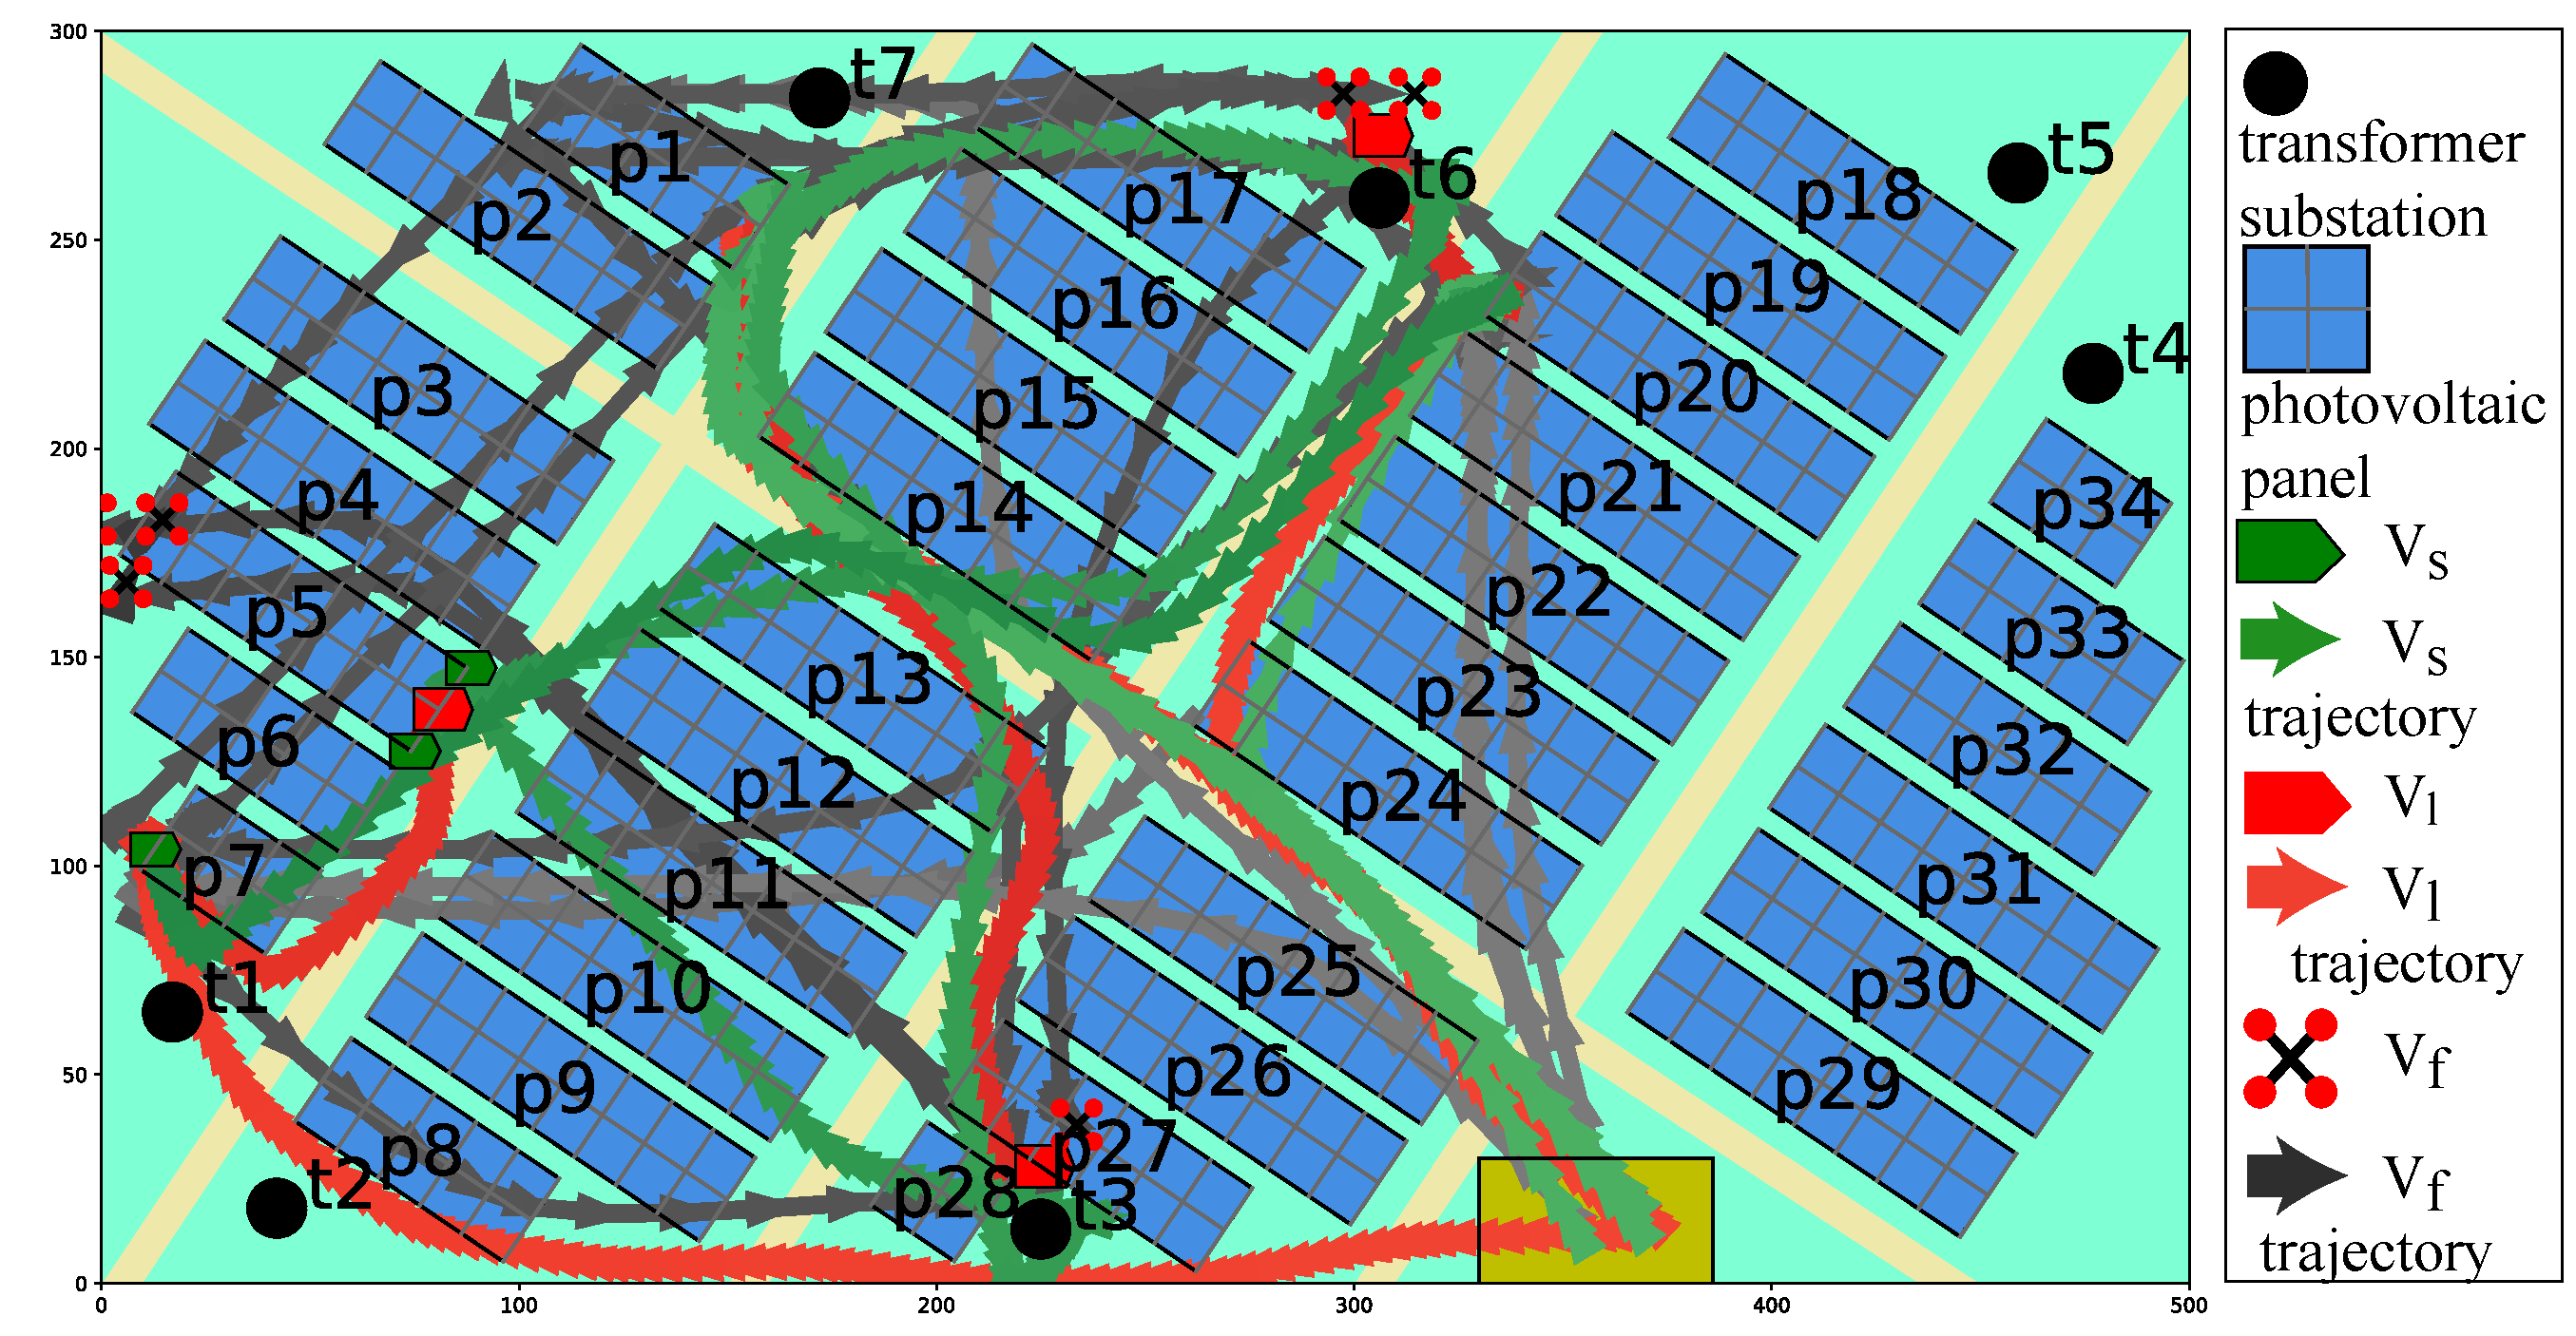
\includegraphics[scale=0.18]{figures/background3.pdf}
\caption{Simulated PV power station in the numerical study,
  which consists of PV panels~$\texttt{p}_i$, roads,
  inverters/transformers~$\texttt{t}_i$ and base stations~$b$.
  The arrow trajectories are the path of Agent swarm
  executing the LTL formula~$\varphi_{3}$. And the arrow direction
  is the motion direction and the arrow density correspond to the velocity of different agents.}
\label{fig:workspace}
\end{figure}
%==============================

%==============================
\subsubsection{Workspace Description}\label{subsubsec:ws}

Consider a group of UAVs and UGVs that work within a PV power station for
long-term daily maintenance.
As shown in Fig.~\ref{fig:workspace},
the station consists of mainly three parts: PV panels, roads,
inverter/transformer substations and the robot base station.
These areas of interest are highlighted in Fig.~\ref{fig:workspace}:
different areas of PV panels are indicated by~$\texttt{p}_1,\cdots,\texttt{p}_{34}$;
the base station for all agents is denoted by~$\texttt{b}$;
the transformer substations are indicated by~$\texttt{t}_1,\cdots,\texttt{t}_7$.

Furthermore, there are one type of UAVs and two types of UGVs.
The UAVs are quadcopters that are capable of fast movement
to inspect the operation condition of PV panels and transformers,
and supervise the maintenance, denoted by~$V_f$.
The UGVs have two sizes: the larger ones can collaborate with other UGVs or UAVs
to clean and repair the PV panels and transformers, named~$V_l$;
the smaller ones can travel more freely, e.g., under the PV panels and between
the transformers,
in order to mow grass or sweep debris within these narrow areas, named~$V_s$.
As a result, different types of robots have different motion
model~$\mathcal{G}_n$ as described in Sec.~\ref{subsec:multi-agent}
and distinctive action models.
The traveling time among the regions of interest is estimated by the route
distance and their respective speed.
Descriptions of these regions of interest and robot actions are summarized in
Table.~\ref{fig:symbols}.
Note that some actions can be performed alone while some require direct
collaboration of several agents,
e.g., one $V_s$ can sweep debris under the PV panel while one $V_l$
and one $V_f$ are required to wash dirt off the surface of PV panels.



%==============================
\subsubsection{Task Description}\label{subsubsec:task}

For the nominal scenario, we consider a system of moderate size,
including $12$ agents: 6 $V_f$, 3 $V_l$ and 3 $V_s$.
Scalability analysis to larger systems are performed later in Sec.~\ref{subsubsec:scalable}.
Moreover, we consider the following three tasks with increasing complexity.


%==============================
\begin{table}[t]
 \centering
\caption{Description of related regions and agent actions.}
\label{fig:symbols}
\begin{tabular}{|c|m{0.5\columnwidth}|c|}\hline
\textbf{Proposition} & \textbf{Description}\centering & \textbf{Duration} [s]\\ \hline
$\texttt{p}_1,\cdots,\texttt{p}_{34}$ & $34$ PV panels. & $\backslash$ \\ \hline
$\texttt{b}$ & Base stations for all agents to park and charge. & $\backslash$ \\ \hline
$\texttt{t}_1,\cdots,\texttt{t}_7$ & $7$ transformers. & $\backslash$ \\ \hline
$\texttt{temp}_{\texttt{p}_i,\texttt{t}_i}$ &
Measure temperature of panel~$\texttt{p}_i$ and transformer $\texttt{t}_i$.
Requires one~$V_f$. & 10 \\ \hline
$\texttt{sweep}_{\texttt{p}_i}$& Sweep debris around any panel~$\texttt{p}_i$.
Requires one $V_s$. & 190\\ \hline
$\texttt{mow}_{\texttt{p}_i,\texttt{t}_i}$ &
Mow the grass under panel~$\texttt{p}_i$ or transformer~$\texttt{t}_i$.
Requires one $V_s$. & 190\\ \hline
$\texttt{fix}_{\texttt{t}_i}$ &
Fix malfunctional transformer~$\texttt{t}_i$.
Requires one $V_l$ and one $V_s$ & 72\\ \hline
$\texttt{repair}_{\texttt{p}_i}$ &
Repair broken panel~$\texttt{p}_i$.
Requires one $V_s$ to repair and two $V_f$ to guide. & 576\\ \hline
$\texttt{wash}_{\texttt{p}_i}$ &
Wash the dirt off panel~$\texttt{p}_i$.
Requires one $V_l$ to wash and one $V_f$ to monitor the progress. & 565\\ \hline
$\texttt{scan}_{\texttt{p}_i,\texttt{t}_i}$ &
Build 3D models of panel~$\texttt{p}_i$ or transformer~$\texttt{t}_i$
for inspection. Requires three $V_f$. & 95\\ \hline
\end{tabular}
\end{table}
%==============================

\textbf{Task One}: A simple and regular maintenance task,
which includes to repair the panel~$\texttt{p}_{31}$,
fix the transformer~$\texttt{t}_6$, wash the panel~$\texttt{p}_{15}$,
and mow grass around the transformer~$\texttt{t}_8$.
This task can be specified as the following LTL formulas:
\begin{equation}\label{eq:task1}
  \begin{aligned}
\varphi_1 = & \texttt{repair-scan}_{\texttt{p}_{31}}
\wedge \texttt{fix-scan}_{\texttt{t}_{6}}\\
&\wedge \Diamond \texttt{wash}_{\texttt{p}_{15}}
\wedge \Diamond \texttt{mow}_{\texttt{p}_8},
\end{aligned}
\end{equation}
where the ``repair and scan'' and ``fix and scan'' routines are defined as follows:
\begin{equation*}
\begin{aligned}
  \texttt{repair-scan}_{\texttt{p}_i}=\,
  & \Diamond \left({\texttt{repair}_{\texttt{p}_i}}
  \wedge \Diamond {\texttt{scan}_{\texttt{p}_i}}\right)\\
&\wedge \Box \left(\texttt{repair}_{\texttt{p}_i}
\rightarrow \lnot \texttt{scan}_{\texttt{p}_i}\right);\\
\texttt{fix-scan}_{\texttt{t}_i} =\,
& \Diamond \left({\texttt{fix}_{\texttt{t}_i}}
\wedge \Diamond {\texttt{scan}_{\texttt{t}_i}}\right)\\
&\wedge \Box \left(\texttt{fix}_{\texttt{t}_i}
\rightarrow \lnot \texttt{scan}_{\texttt{t}_i}\right),
\end{aligned}
\end{equation*}
which specifies that a scanning is required \emph{after}
a panel is repaired or a transformer is fixed.
This task can be clearly divided into several parallel sub-tasks
that can be executed simultaneously and independently.
The location of these subtasks are chosen across the workspace
thus a coordination strategy to minimize completion time is crucial for the task.

\textbf{Task Two}: A complex maintenance task that involves several
sequential routines.
It includes to deep clean several panels and monitor
the temperature of several transformers.
It can be expressed as the following LTL formulas:
\begin{equation}\label{eq:task2}
    \varphi_2 = (\bigwedge_{i=11,20}
    \texttt{deep-clean}_{\texttt{p}_i} ) \wedge  \Diamond
    \texttt{temp}_{\texttt{t}_4},
\end{equation}
where the ``deep cleaning'' routine consists of three steps:
wash the panel,  mow the grass, and finally sweep the debris:
\begin{equation*}
  \begin{aligned}
    \texttt{deep-clean}_{\texttt{p}_i} &= \Diamond (
    \texttt{wash}_{\texttt{p}_i} \wedge\Diamond \texttt{scan}_{\texttt{p}_i} \\
    & \wedge \Diamond
    \left(\texttt{mow}_{\texttt{p}_i} \wedge
    \Diamond \texttt{sweep}_{\texttt{p}_i} \right))\\
    & \wedge \Box \left((\texttt{wash}_{\texttt{p}_i} \lor \texttt{mow}_{\texttt{p}_i})
    \rightarrow \lnot \texttt{sweep}_{\texttt{p}_i} \right)\\
    & \wedge \Box \left( \texttt{wash}_{\texttt{p}_i} \rightarrow
    \lnot \texttt{mow}_{\texttt{p}_i} \right)\\
    &\wedge \Box \left( \texttt{wash}_{\texttt{p}_i} \rightarrow
    \lnot \texttt{scan}_{\texttt{p}_i} \right),
  \end{aligned}
\end{equation*}
which indicates that for safety reasons the deep cleaning should be performed
in sequence of washing, mowing and sweeping.
Clearly, compared with Task One, Task Two contains more constraints on the
sequential order of subtasks, thus requiring more synchronization during
execution.
However, since there are many panels that require deep cleaning
and the temperature of many transformers should be measured,
these processes can be performed in parallel.
Thus most agents especially the UAVs are responsible for more than one subtasks,
which is quite different from Task One.

\textbf{Task Three}: As the most complex task, Task Three combines the previous
two tasks. Namely, it consists of all possible maintenance tasks,
including the repair and fixation of panels and transformers,
the deep cleaning of panels, and the monitoring of panels and transformers,
as the following formulas:
\begin{equation}\label{eq:task3}
  \begin{aligned}
    &\varphi_3 =
    (\bigwedge_{i=1,5} \texttt{repair-scan}_{\texttt{p}_i})
    \wedge (\bigwedge_{i=17,24}\Diamond \texttt{temp}_{\texttt{p}_{i}})\\
     &\wedge
     (\bigwedge_{i=3,6} \texttt{fix-scan}_{\texttt{t}_i})  \wedge
     (\bigwedge_{i=7,20} \texttt{deep-clean}_{\texttt{p}_i})
  \end{aligned}
\end{equation}
of which the routines are defined in~\eqref{eq:task1} and~\eqref{eq:task2}.
Clearly, for a team of~$12$ agents, Task Three with~$18$ sub-tasks is significantly
much more complex
than the previous two tasks, and thus much harder to coordinate the whole system.

%===========================
\begin{figure}[t!]
	\begin{minipage}[t]{0.5\linewidth}
		\centering%
		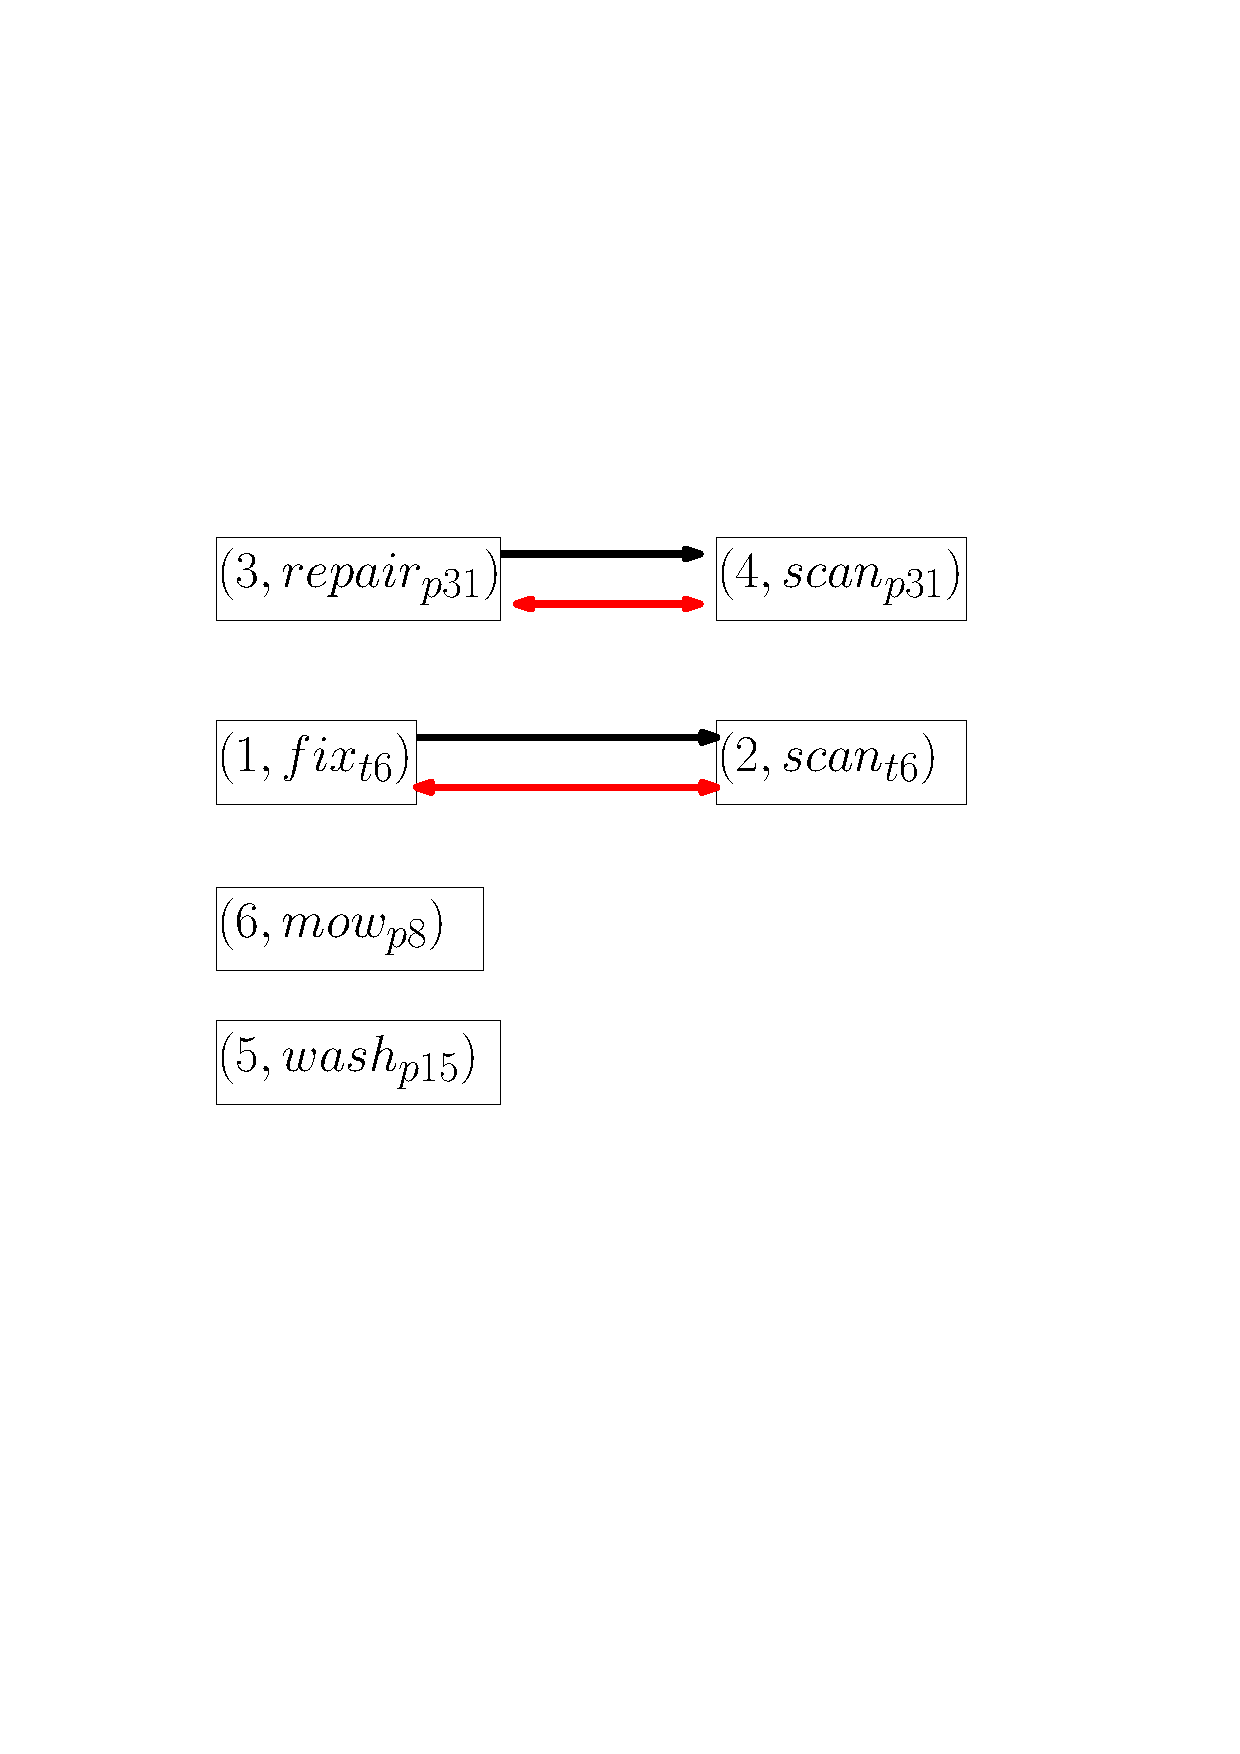
\includegraphics[height = 0.6 \textwidth]{figures/simulation/task1/ipe_poset_graph.pdf}
	\end{minipage}%
	\begin{minipage}[t]{0.5\linewidth}
		\centering%
		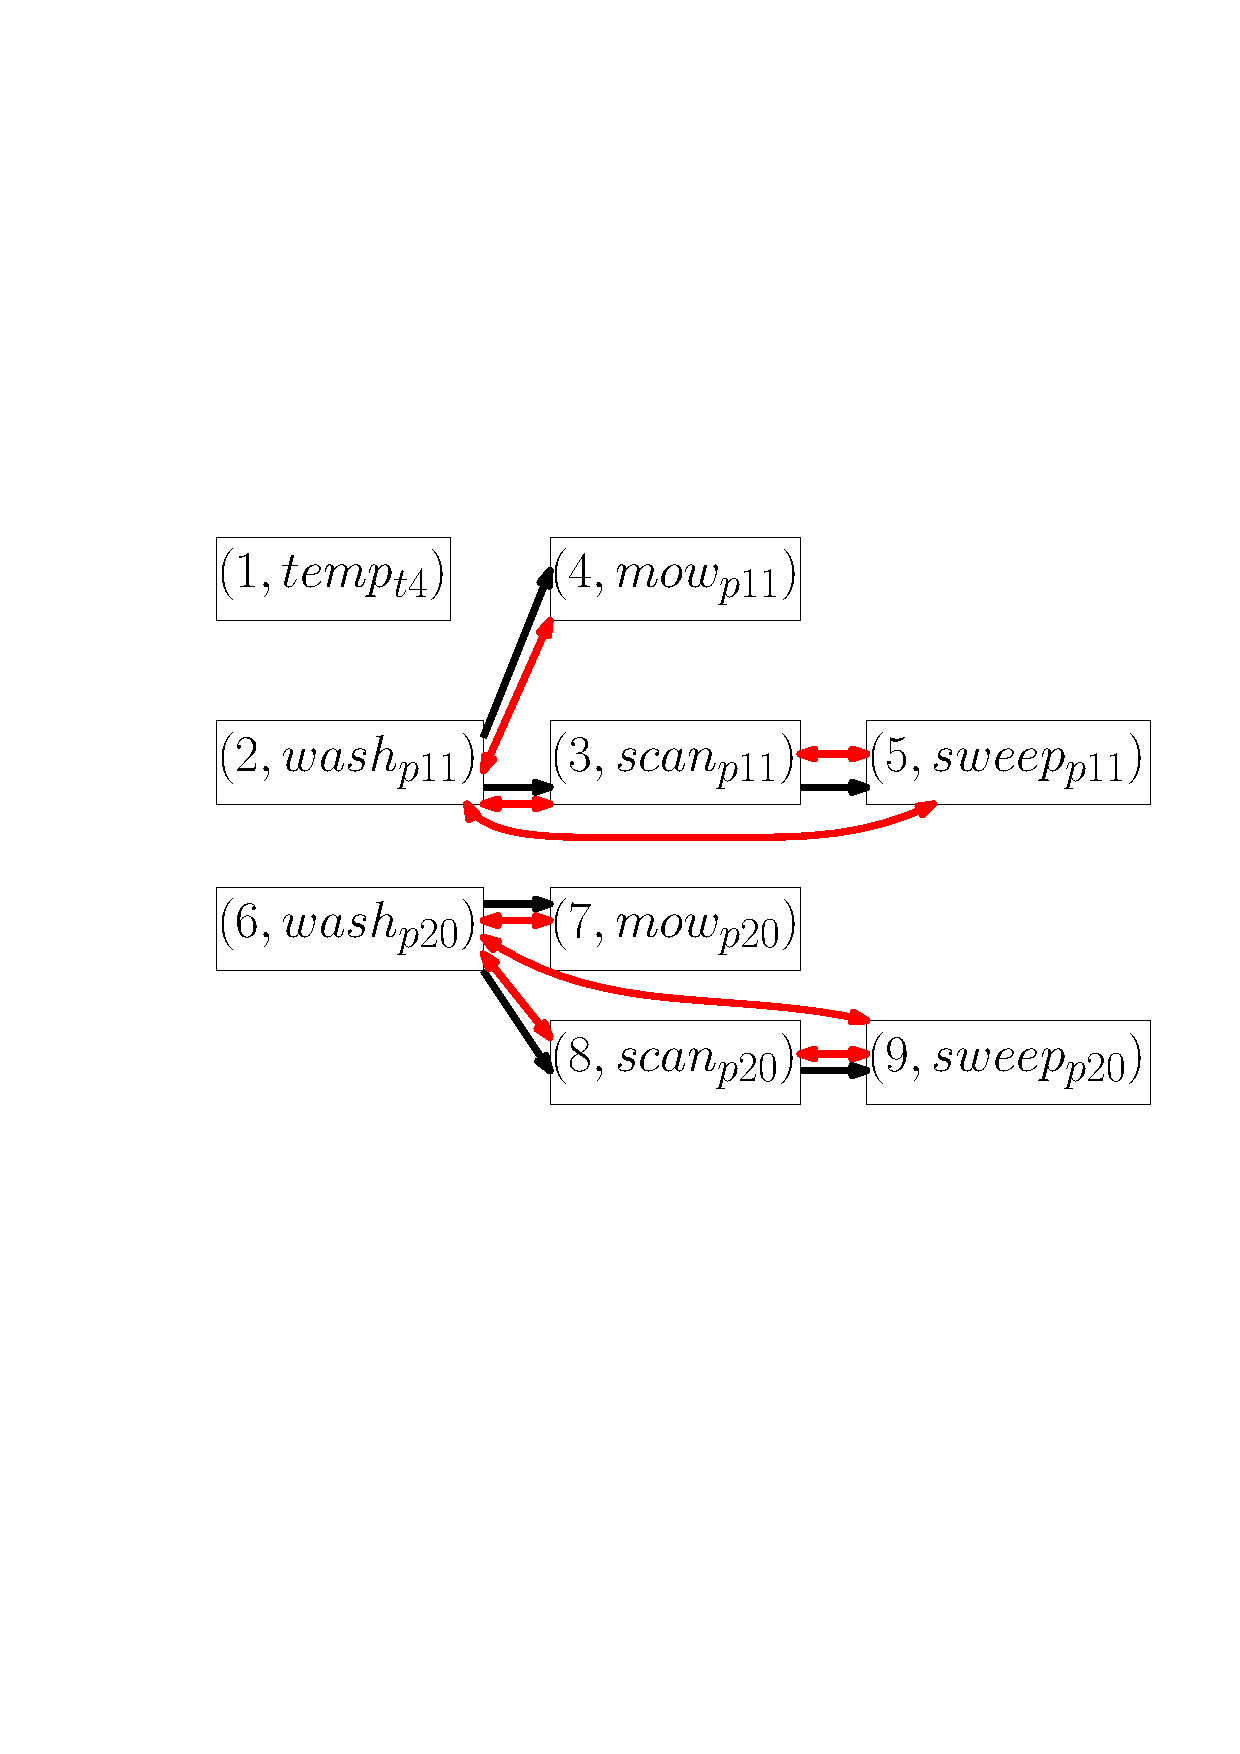
\includegraphics[height = 0.6 \textwidth]{figures/simulation/task2/ipe_poset_graph.pdf}
		\label{fig:poset_graph1}
	\end{minipage}%
	\caption{\textbf{Left}: Poset graph of task $\varphi_1$;
          \textbf{Right}: Poset graph of task $\varphi_2$.
          The relations~$\preceq_\varphi,\, \neq_{\varphi}$ are marked
          by black and red arrows, respectively.}
       \label{fig:task12-posets}
\end{figure}
%===========================

%========================================
\subsubsection{Results}\label{subsubsec:results}
In this section, we present the results of the proposed method for
the above tasks, including the computation of posets,
task assignment via the BnB search algorithm, and the task execution results.

\textbf{Task One}:
The NBA~$\mathcal{B}_{\varphi}$ associated with task one in~\eqref{eq:task1}
contains~$54$ states and~$430$ edges. And the pruning step reduced $1.9\%$ states
and $56\%$ edges within $0.25$ second. The Alg.~\ref{alg:compute-poset} explores
 $180$ accepting runs in $0.04$ second and finds only one poset $P_{\varphi}$ with $6$ subtasks
that can describe all the accepting runs in~$L_\varphi$.
That means we can use $P_{\varphi}$ to completely replace the $\mathcal{B}_{\varphi}$ without
losing any message.


%===========================
\begin{figure}[t!]
\centering%
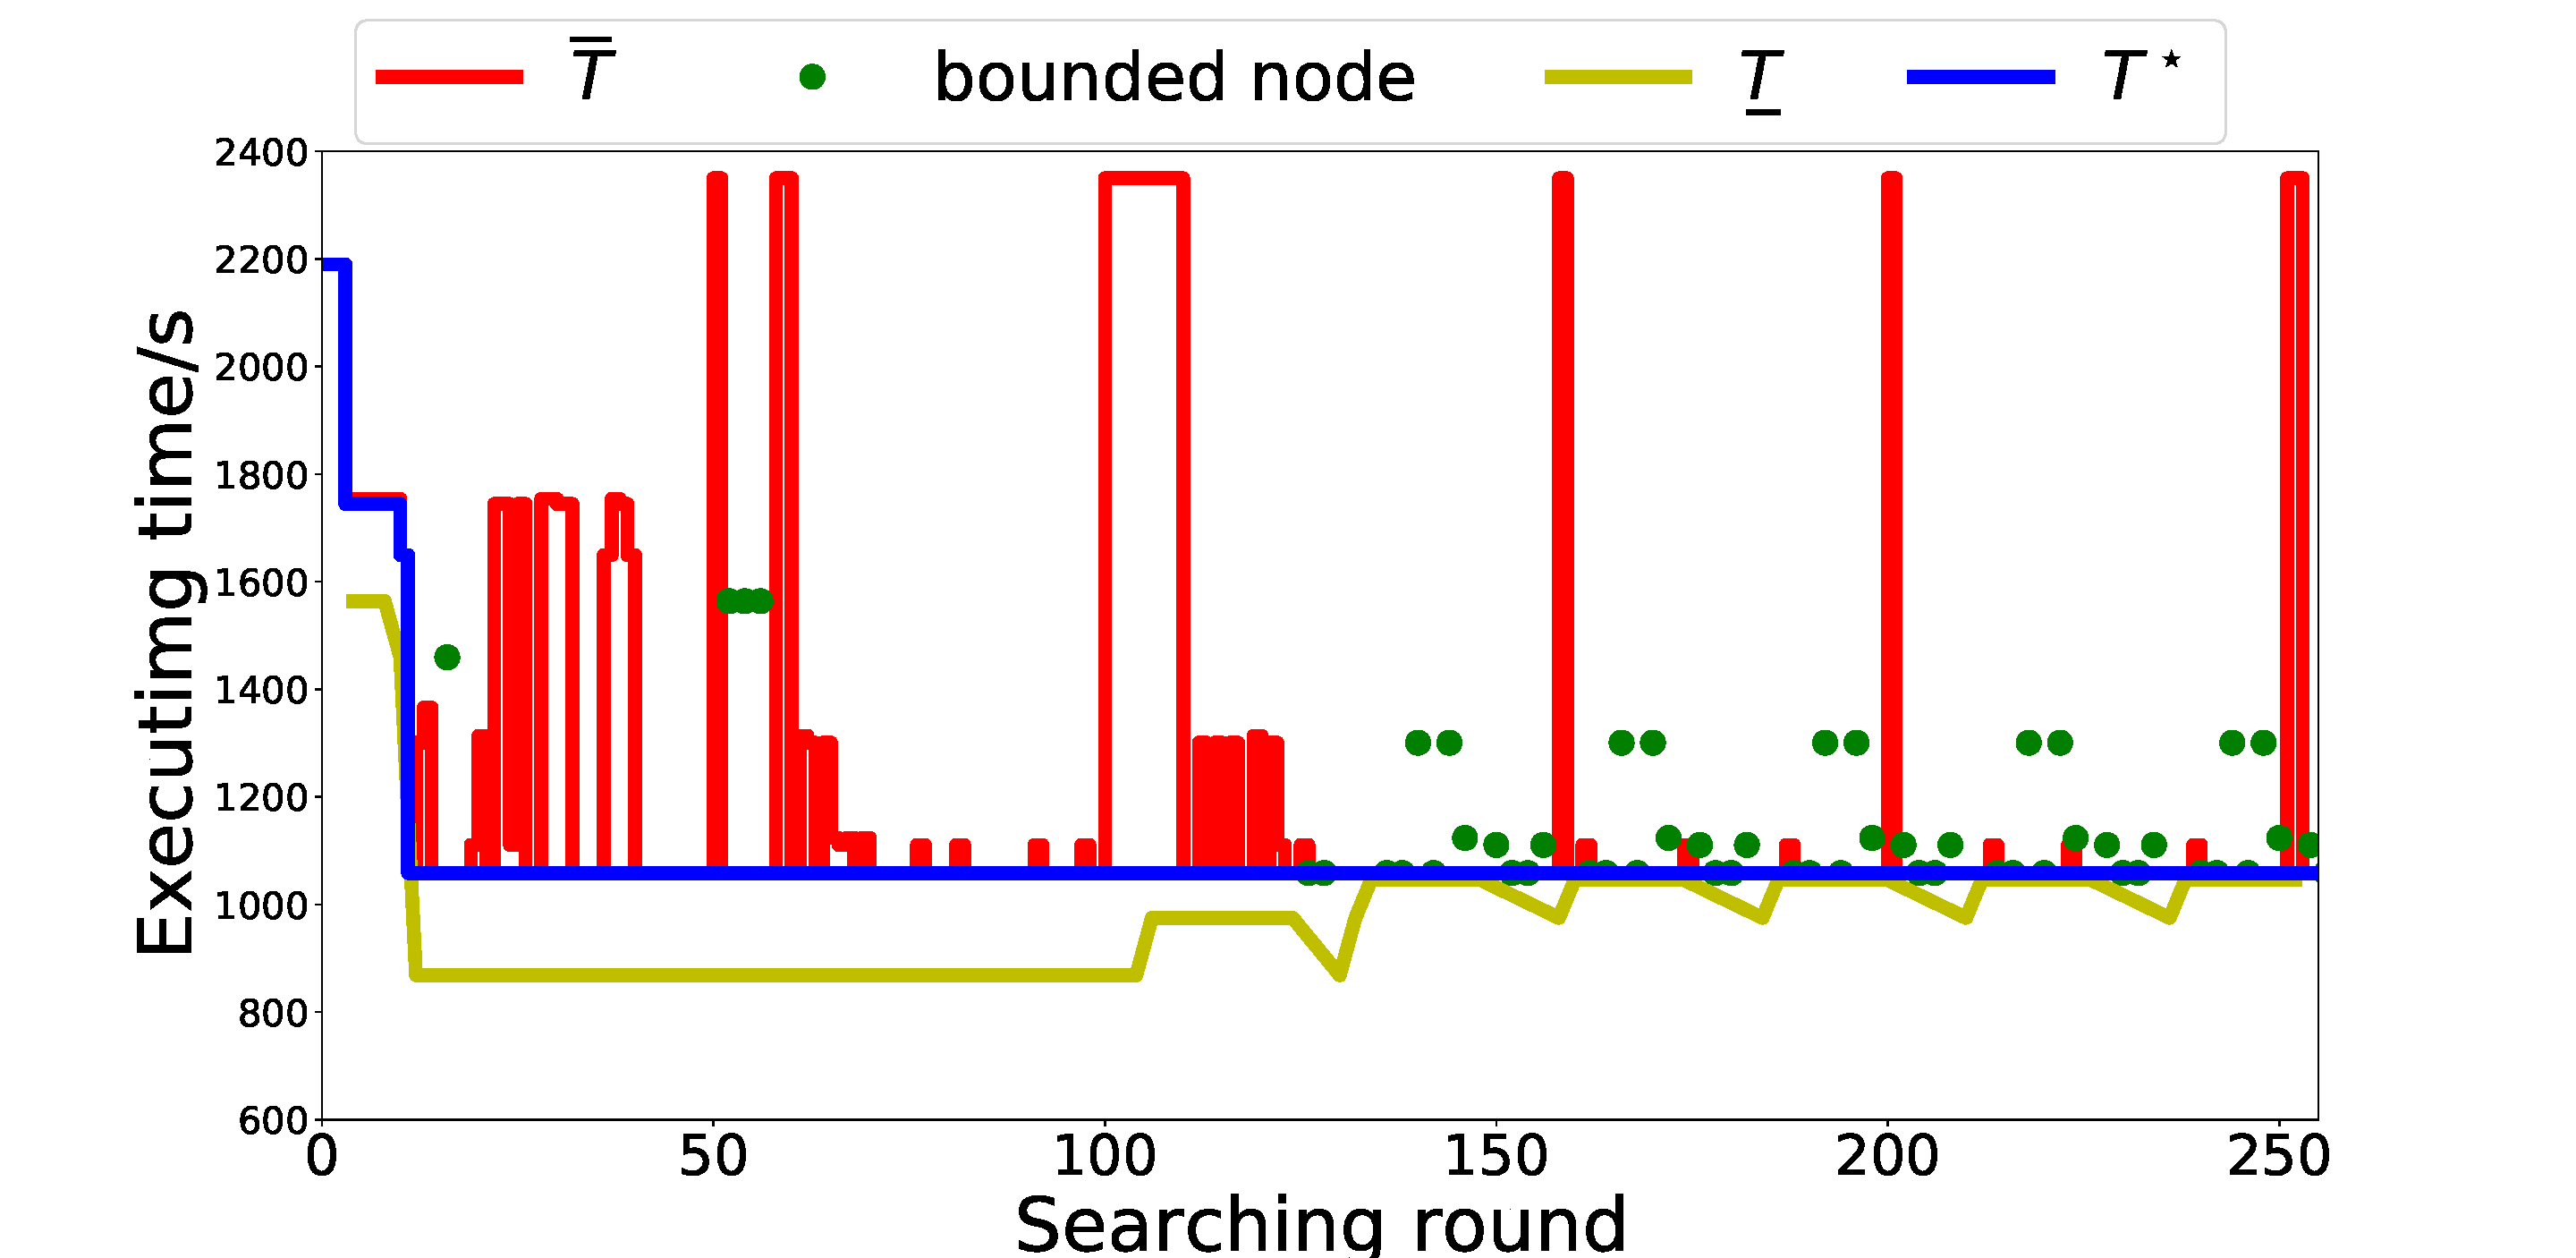
\includegraphics[width = 0.48\textwidth]{figures/simulation/task2/bnb_search3.pdf}
\caption{Illustration of the upper and lower
bounds~$\overline{T}_\nu,\,\underline{T}_\nu$, and the optimal value~$T^\star$,
along with the BnB search process.}
\label{fig:task2-bnb}
\end{figure}
%===========================

This poset~$P_{\varphi}$ constructed of~$6$ subtasks,
and the partial relations $\preceq_{\varphi}$ has $2$ elements,
and $\neq_{\varphi}$ has $2$ elements.
 Note that~$\mathcal{L}(P_\varphi)$ is equal to $\mathcal{L}(\mathcal{B}_{\varphi}^-)$ so that
 this one poset provides a compact representation of all the allowed words
 of formula~$\varphi_{1}$.
The corresponding diagram of poset~$\mathcal{G}_{P_\varphi}$ is shown in
Fig.~\ref{fig:task12-posets}, where the subtasks are separated into four
parallel branches and connected by their partial relations.
Clear correspondences can be found from the LTL formula to the partial relations:
$\Diamond ({\texttt{fix}_{\texttt{t}_6}}\wedge \Diamond {\texttt{scan}_{\texttt{t}_6}})$
maps to $\texttt{fix}_{\texttt{t}_6}\preceq_{\varphi} \texttt{scan}_{\texttt{t}_6}$;
$ \Diamond({\texttt{repair}_{\texttt{p}_{31}}}\wedge \Diamond {\texttt{scan}_{\texttt{p}_{31}}})$
to $\texttt{repair}_{\texttt{p}_{31}}\preceq_{\varphi} \texttt{scan}_{\texttt{p}_{31}}$;
$\Box (\texttt{fix}_{\texttt{p}_i}\rightarrow \lnot \texttt{scan}_{\texttt{p}_i})$ to
$\texttt{fix}_{\texttt{t}_6}\neq_{\varphi} \texttt{scan}_{\texttt{t}_6}$;
 and $\Box (\texttt{repair}_{\texttt{p}_i}\rightarrow \lnot \texttt{scan}_{\texttt{p}_i})$ to
 $\texttt{repair}_{\texttt{p}_{31}}\neq_{\varphi} \texttt{scan}_{\texttt{p}_{31}}$.
Visualization of the final assignment is omitted here due to limited space,
and given in the supplementary file.
Then, during the task assignment,
the first valid solution is found in~$0.24s$.
Afterwards, at~$t=0.55s$, a node is reached and its estimated lower
bound is larger than current upper bound, and thus cut off the search tree.
Overall, around~$33\%$ of visited nodes are cut off,
which clearly shows the benefits of the ``bounding'' mechanism.
Then, the estimated upper-bound rapidly converged
to the optimal solution in~$3.12s$ with exploring~$21$ nodes.
This is due to the branching efficiency during the BnB search,
by using the estimated lower bounds as heuristics.
Lastly, the whole search tree is exhausted after more than~$10$ hours
due to the complexity of the question.
In the optimal task assignment, all~$6$ $V_f$ are deployed.
All agents are assigned to only one task except~$V_{s12}$, $V_{f6}$
which have two subtasks.
It can be seen that tasks without partial constraints
such as~$\texttt{repair}_{\texttt{P}_{31}}, \texttt{repair}_{\texttt{P}_{15}}$
are distributed to different agents. The tasks with partial constrains
are always satisfied, as shown by the marked triangles.
The makespan is determined by the execution of~$\texttt{repair}_{\texttt{P}_{31}},
\texttt{scan}_{\texttt{P}_{31}}$ as $731s$.




%==============================
\begin{figure*}[t!]

  \begin{minipage}[t]{0.22\linewidth}
   \centering %
	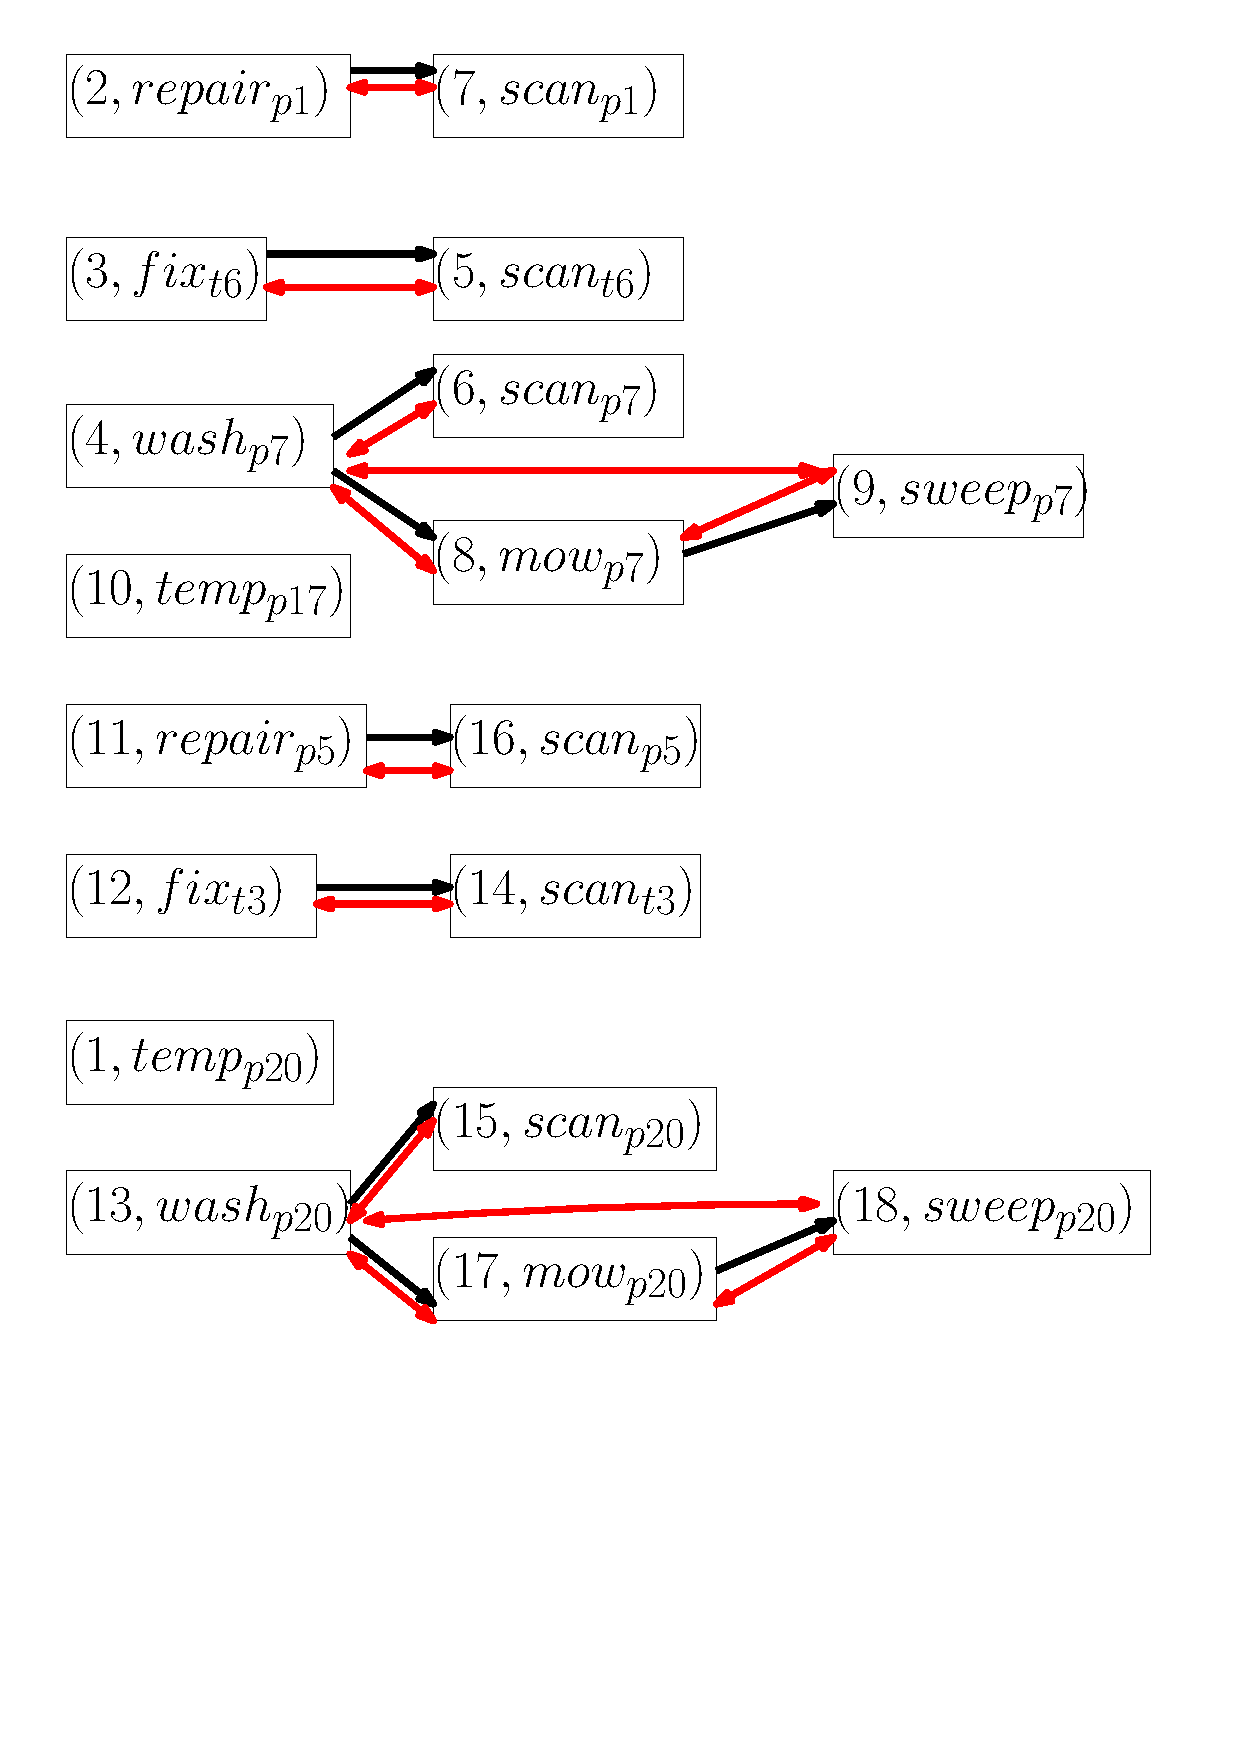
\includegraphics[height =1.2\textwidth]{figures/simulation/task3/ipe_poset_graph.pdf}

\end{minipage}%
  \begin{minipage}[t]{0.37\linewidth}
    \centering
	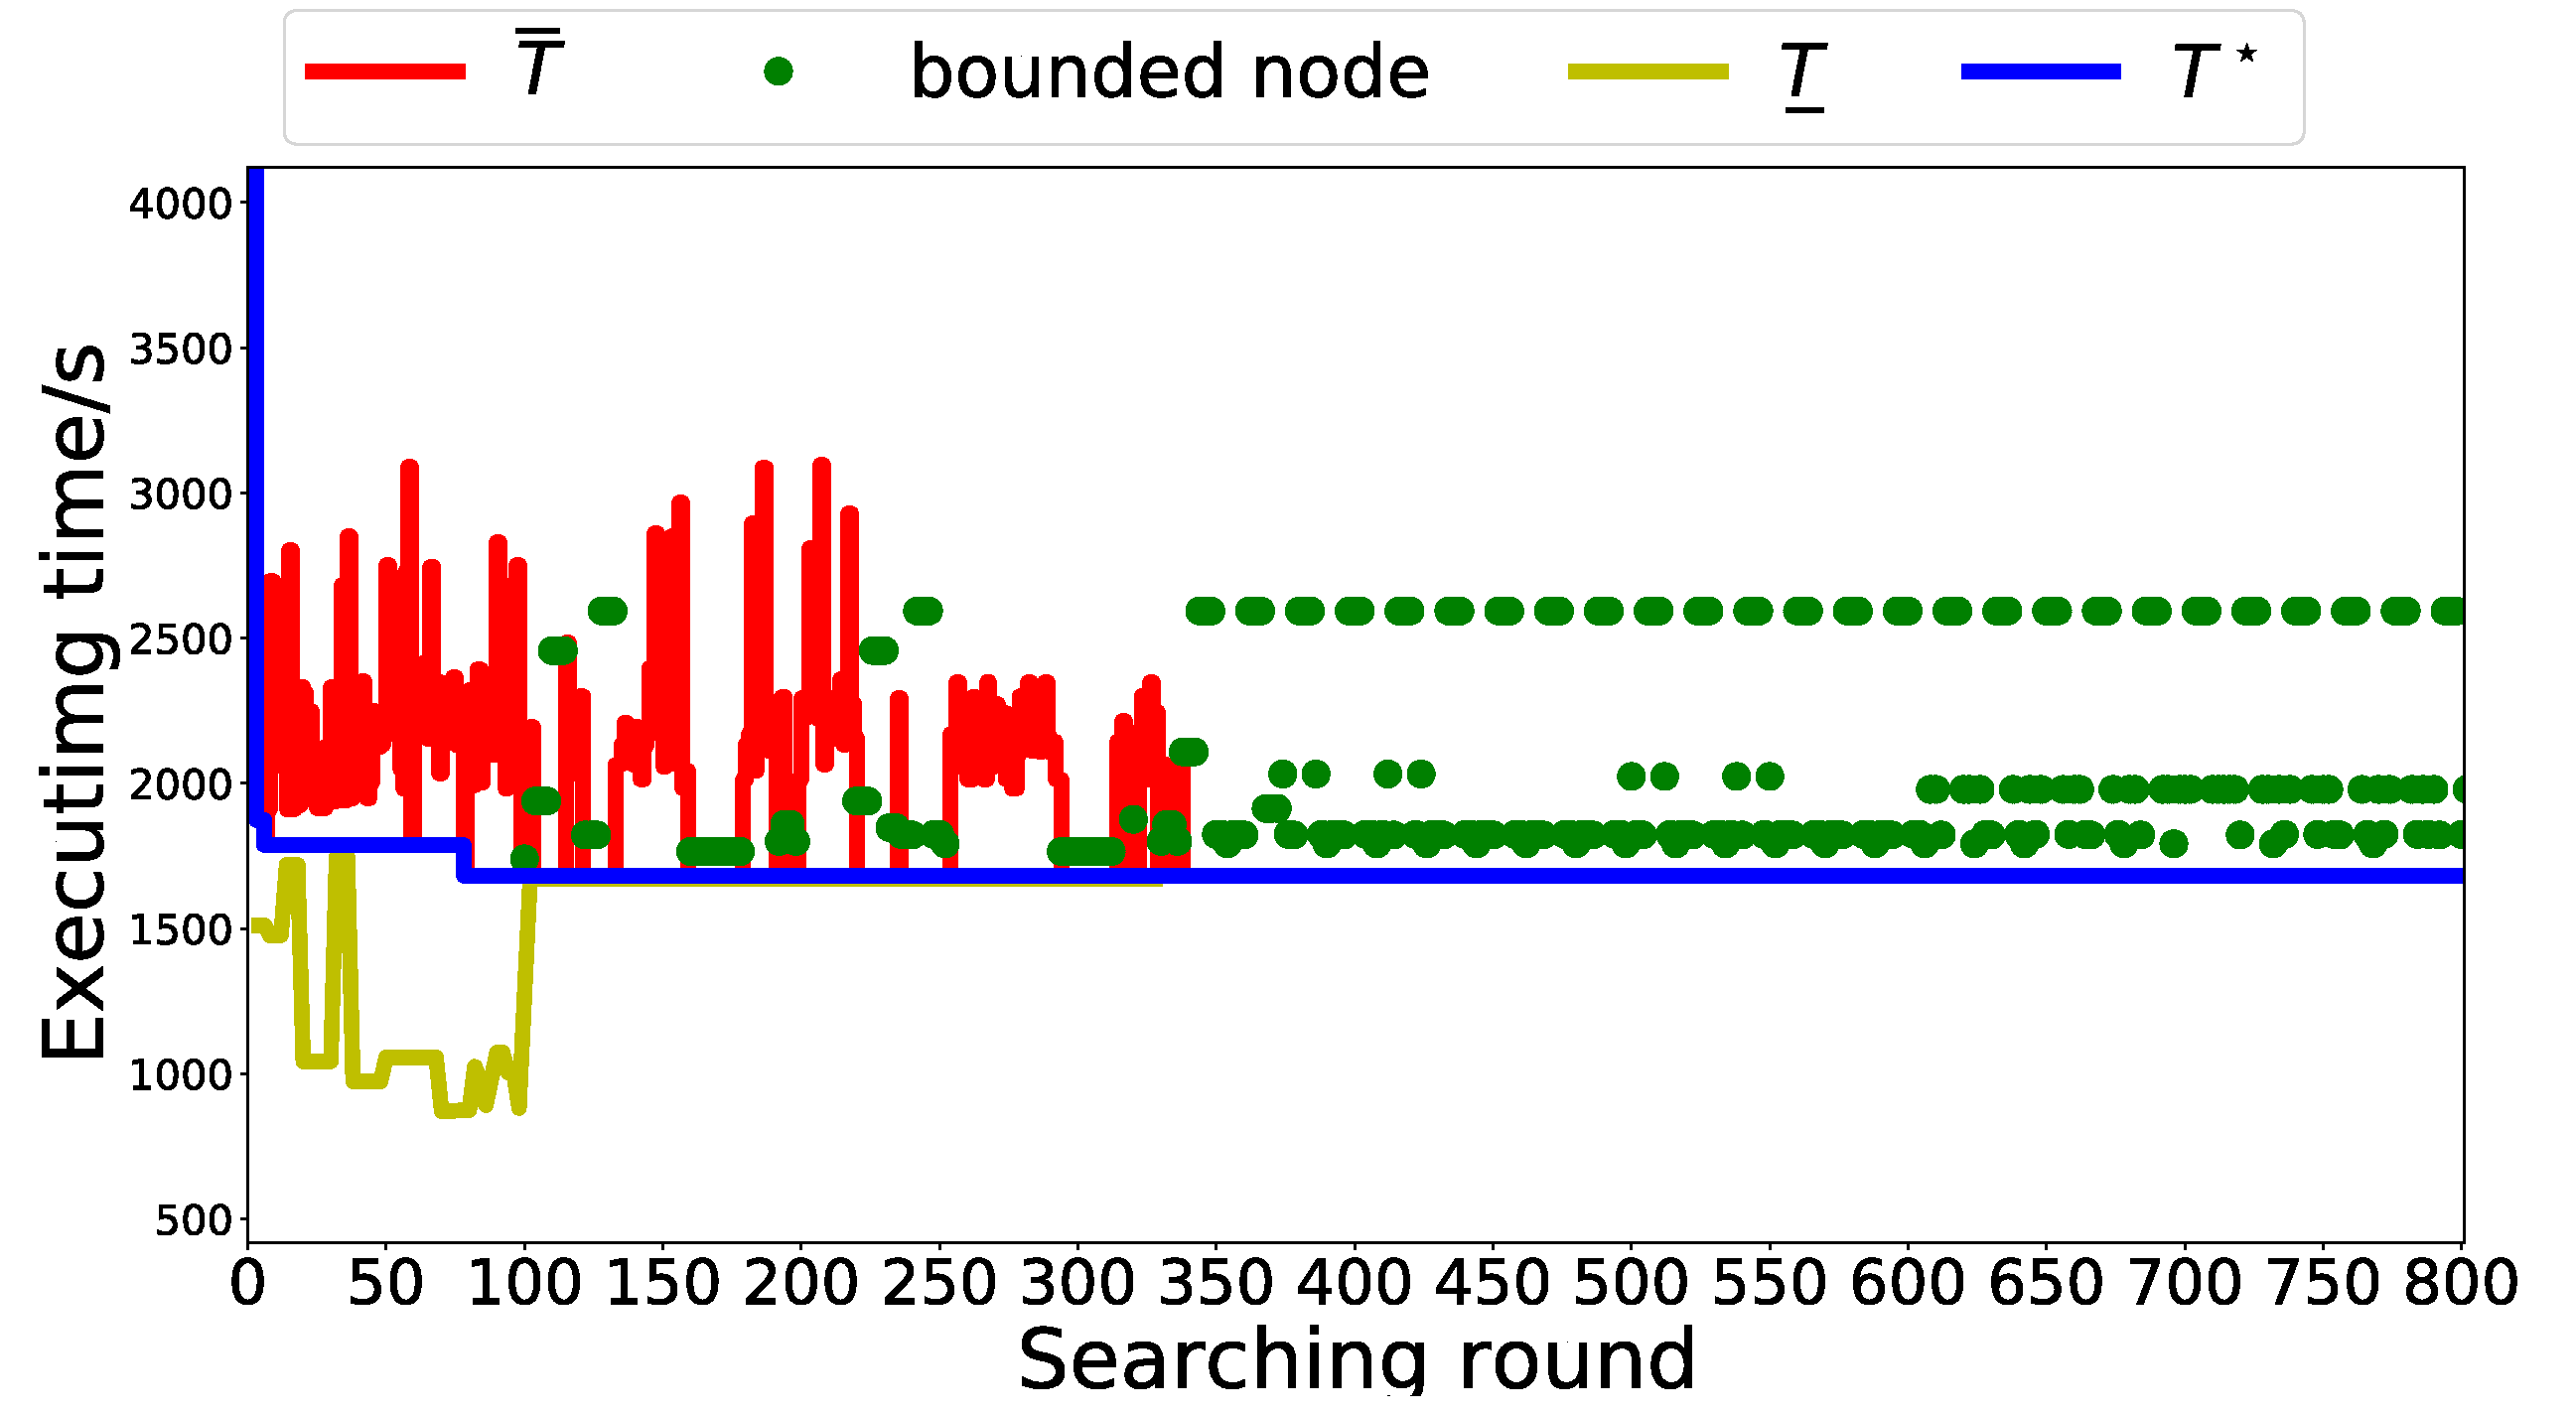
\includegraphics[width =1.10\textwidth]{figures/simulation/task3/bnb_search4.pdf}

\end{minipage}%
  \begin{minipage}[t]{0.4\linewidth}
	\centering
	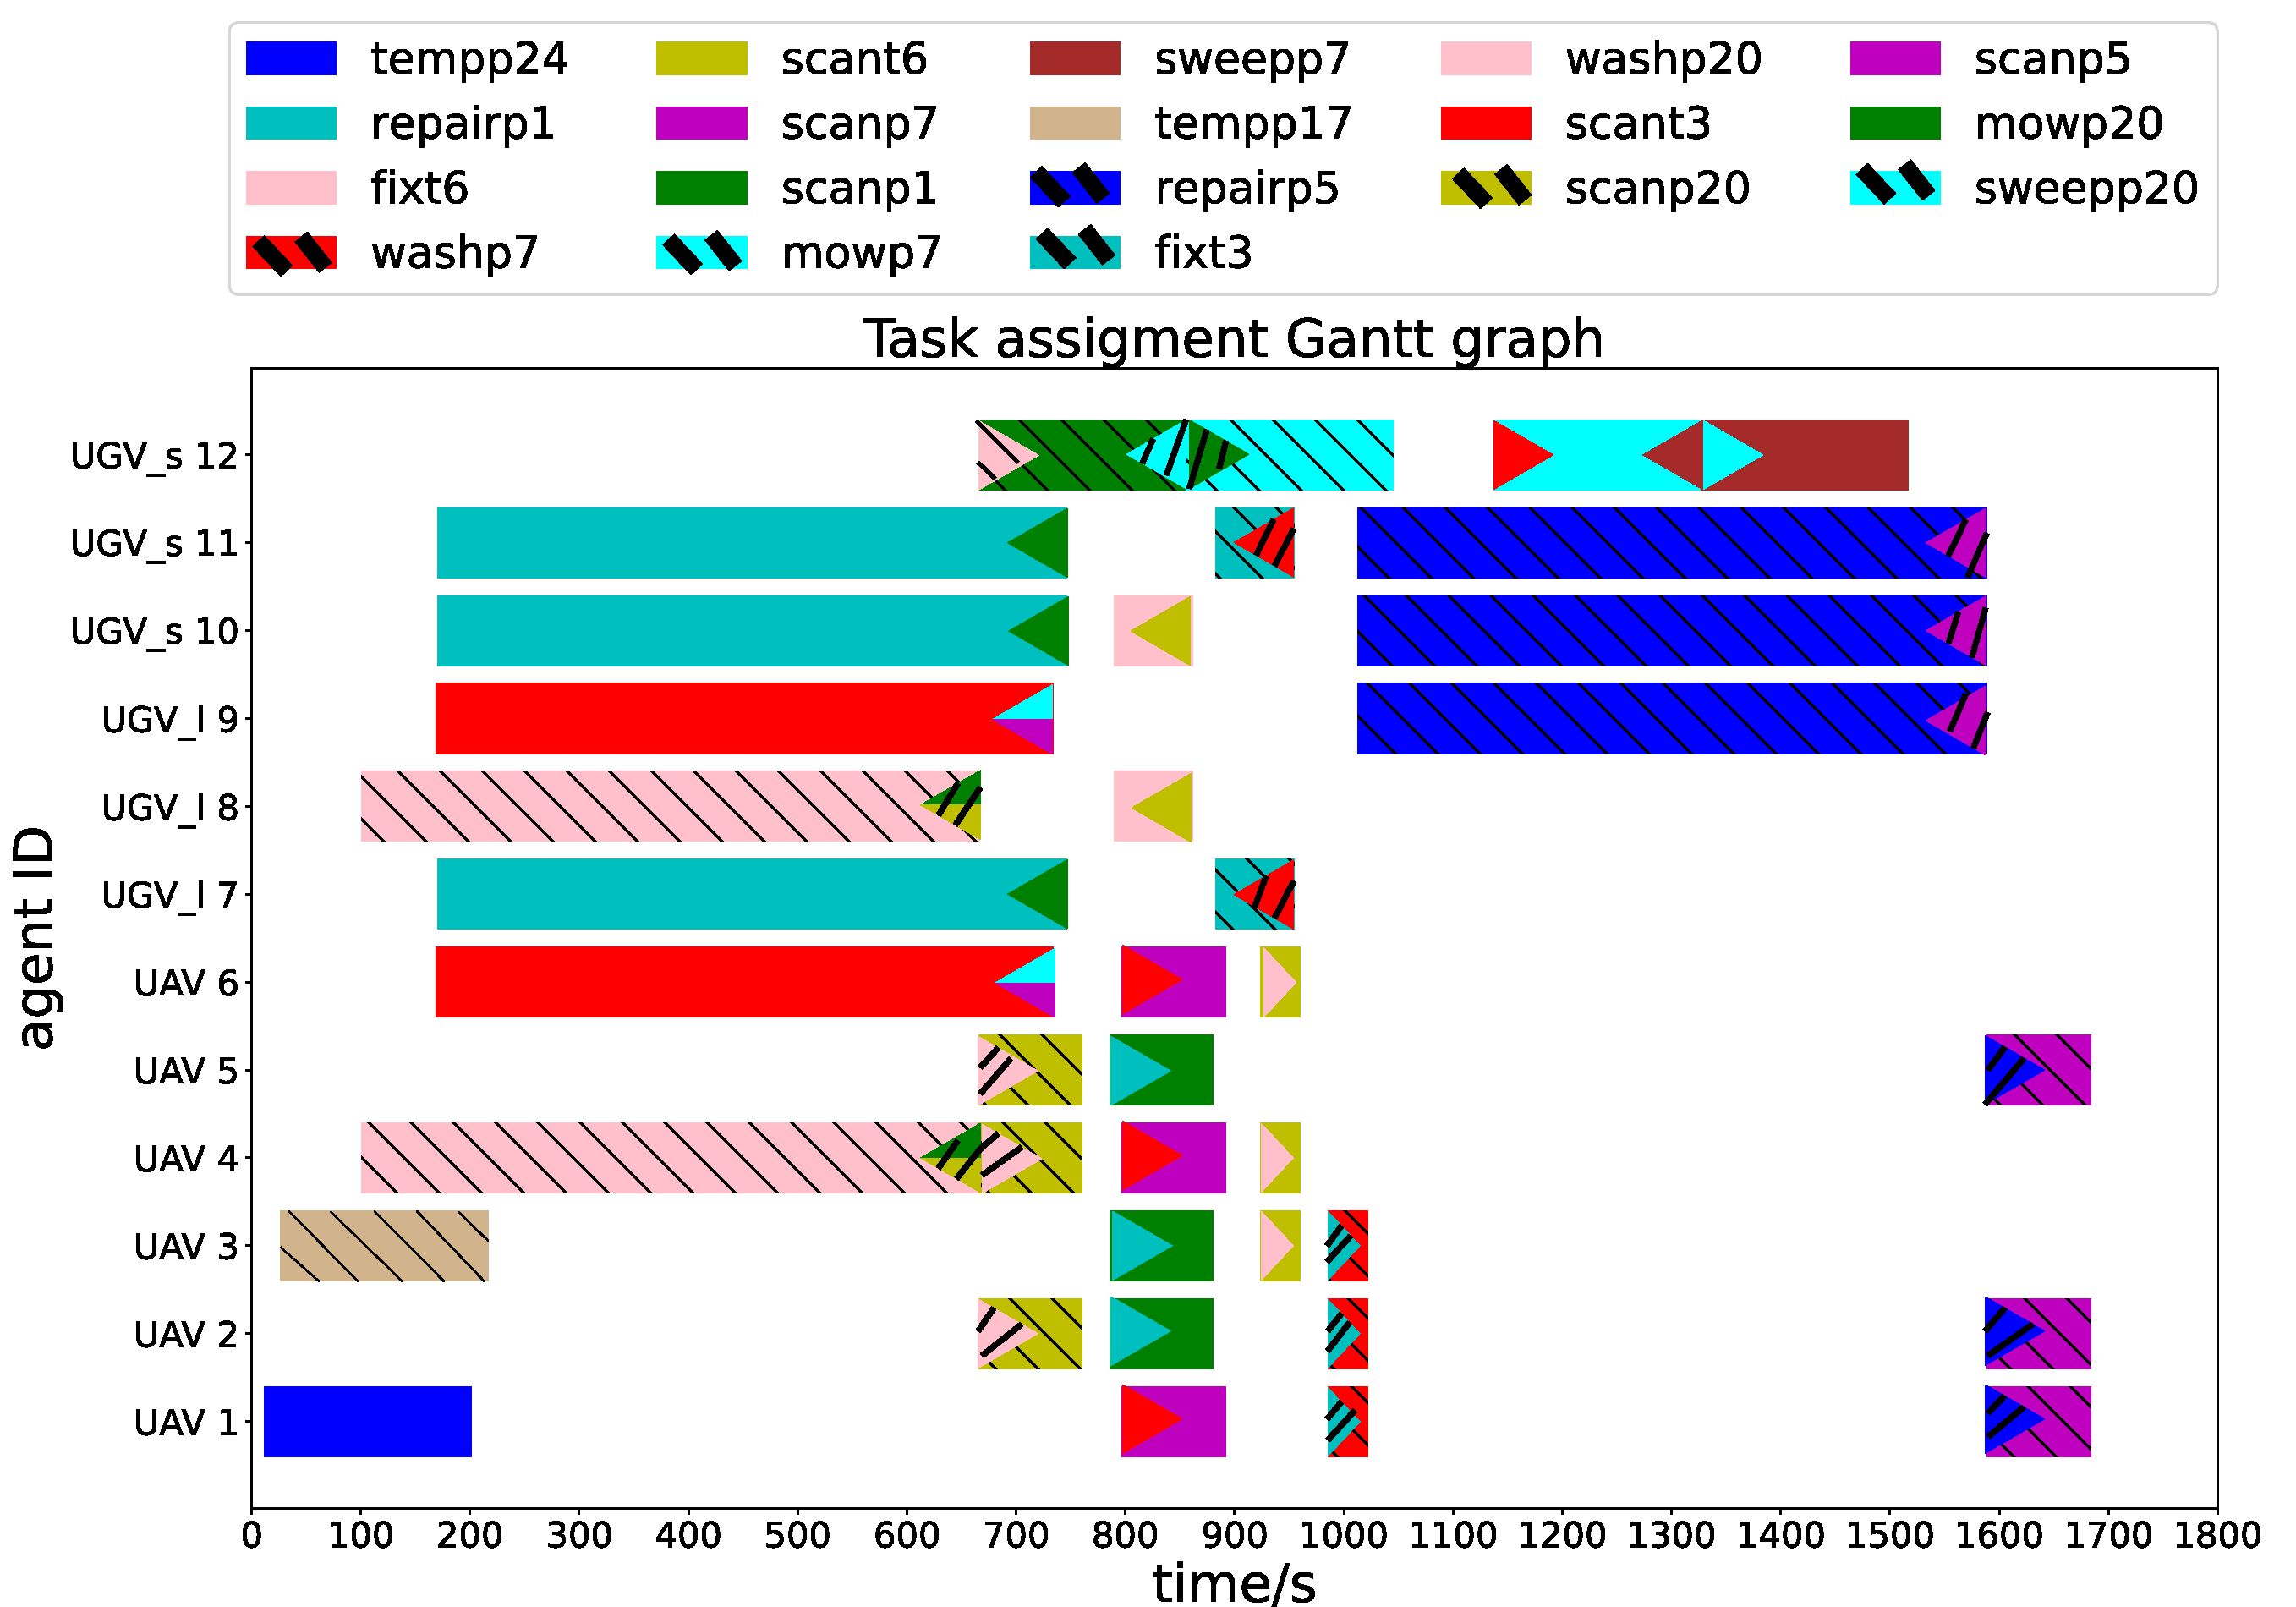
\includegraphics[width = 0.85\textwidth]{figures/simulation/task3/gantt_s0.pdf}

\end{minipage}%
  \caption{\textbf{Left}: Poset graph associated with task~$\varphi_3$;
    \textbf{Middle}: Evolution of the upper and lower
    bounds~$\overline{T}_\nu,\,\underline{T}_\nu$,
    and the optimal value~$T^\star$ during the BnB search process;
    \textbf{Right}: Gantt graph of the optimal task assignment,
    where the tasks with partial constrains are marked by triangles.}
  \label{fig:task3-results}
\end{figure*}
%==============================

\textbf{Task Two}:
Compared with Task One,
task two contains more ordering constraints, e.g.,
the sub-task~$\texttt{deep-clean}_{\texttt{p}_i}$ requires
that~$5$ different subtasks are executed in certain sequences.
The associated NBA~$\mathcal{B}_{\varphi_2}$ is much larger
with~$216$ states and~$2255$ edges,
After pruning, it is reduced to~$203$ states and $1524$ edges in~$4.3s$.
Via Alg.~\ref{alg:compute-poset},
$8$ posets are found after exploring $6870$ accepting runs in~$31.6s$,
and the first poset is obtained in~$4.6s$.
As shown in Fig.~\ref{fig:task12-posets},
the poset with the largest language $L(P_{\varphi})=5670$ is chosen,
which means that this poset contains most (around $82.5\%$)
of the accepting runs in $\mathcal{B}^-_{\varphi_2}$.
The poset graph consists of~$3$ independent branches and there are
no relation $\preceq_{\varphi}$ among any two subtasks in different branches.
Moreover, there exist no direct paths from any subtask in
$\texttt{scan}_{\texttt{p}_{11}}$ to any subtask in~$\texttt{mow}_{\texttt{p}_{11}}$.
That means we can execute these subtasks in parallel
which can significantly reduce the makespan of the whole task.

During the task assignment,
the first solution is obtained in $0.35s$ with a makespan~$2189s$.
As shown in Fig.~\ref{fig:task2-bnb},~$11$ nodes are explored by the proposed BnB method and
the optimal solution is found in~$5.3s$ with the optimal makespan~$1058s$.
Since the posets have more ordering constraints,
which reduces the size of solution space and increases the accuracy of the estimation
of the upper and lower bounds,
it actually takes less explorations to find the optimal plan.
For the same reason, the estimated lower and upper bounds are quite close.
Around~$20\%$ of the explored nodes are removed from the search tree
as their estimated lower bounds are larger than the known upper bound,
which are shown as green dots in Fig.~\ref{fig:task2-bnb}.
It is also interesting to see that for some nodes the estimated upper bound
can be quite large,
which however does not effect the best value~$T^\star$
as monotonically decreasing.
Visualization of the final assignment is omitted here
and given in the supplementary file.
The subtasks~$\texttt{wash}_{\texttt{p}_{11}}$ and
$\texttt{wash}_{\texttt{p}_{20}}$ are executed in parallel by
agents~$V_{f2}$, $V_{l2}$ and~$V_{f6}$, $V_{l3}$, respectively.
The slight difference in their starting time is due to the difference
in transition time between regions.
Moreover, it is worth noting that
the subtasks~$\texttt{scan}_{\texttt{p}_{11}}$ and~$\texttt{mow}_{\texttt{p}_{11}}$
both begin at the moment when~$\texttt{wash}_{\texttt{p}_{11}}$ is finished.
It shows that our algorithm can not only handle parallel routines but also
independent subtasks within these routines.
Notice that all UAVs are deployed first to monitor the progress
of~\texttt{wash} routines, then to collaboratively scan the panels.

\textbf{Task Three}:
As the most complex task,
the associated NBA is already too big to compute for the given computer memory
after~$12h$.
Thus, the routines are treated separately for computing their Nabs and then
composed together.
This is allowed as all routines are related to different actions at different
regions.
Afterwards, their posets are derived separately via Alg.~\ref{alg:compute-poset},
and then composed together  while maintaining consistency.
As shown in Fig.~\ref{fig:task3-results},
the poset contains~$18$ subtasks and~$22$ partial constrains.
The subtasks are divided into~$8$ independent branches,
which matches the intuition as each routine corresponds to an independent branch.

During the BnB search,
the first valid solution is recorded in $0.52s$ with a makespan $4330s$.
In total,~$800$ nodes are explored and the optimal solution is obtained
after exploring~$78$ nodes at $37.24s$. And~$70\%$ of the explored nodes
are removed from the search tree.
The overall computation time is increased significantly due to two aspects:
first, the computation time of both upper and lower bounds
increases linearly with the number of subtasks;
second, more nodes are explored due to the increased complexity
of the posets. But we can still
get a suitable solution quickly after exploring $6$ nodes,
of which the upper bound is within $6.5\%$ above the
optimal value.
The optimal assignment is shown in Fig.~\ref{fig:task3-results},
of which the makespan is~$1683$ seconds.
It is noticed that in this case there might be multiple optimal solutions
with the same makespan.
As the makespan is mainly determined by the final sub-task~$\texttt{scan}_{\texttt{P}_5}$.
The UAVs need to wait for a long time until the previous
subtask~$\texttt{repair}_{\texttt{P}_5}$ is finished. Consequently, the relative ordering
of other subtasks such as~$\texttt{scan}_{\texttt{P}_7}$,
~$\texttt{scan}_{\texttt{T}_6}$,~$\texttt{scan}_{\texttt{T}_3}$
does not affect the makespan.
The proposed algorithm always returns the same optimal solution due to the branching
strategy. Lastly, it can be seen that the makespan of the whole task would be reduced
further if more $V_s,\,V_l$ are deployed,
so that the subtask~$\texttt{fix}-\texttt{scan}$ can be executed earlier.
The final assignment is shown in Fig~\ref{fig:task3-results}.
%==============================
\begin{figure}[t!]
	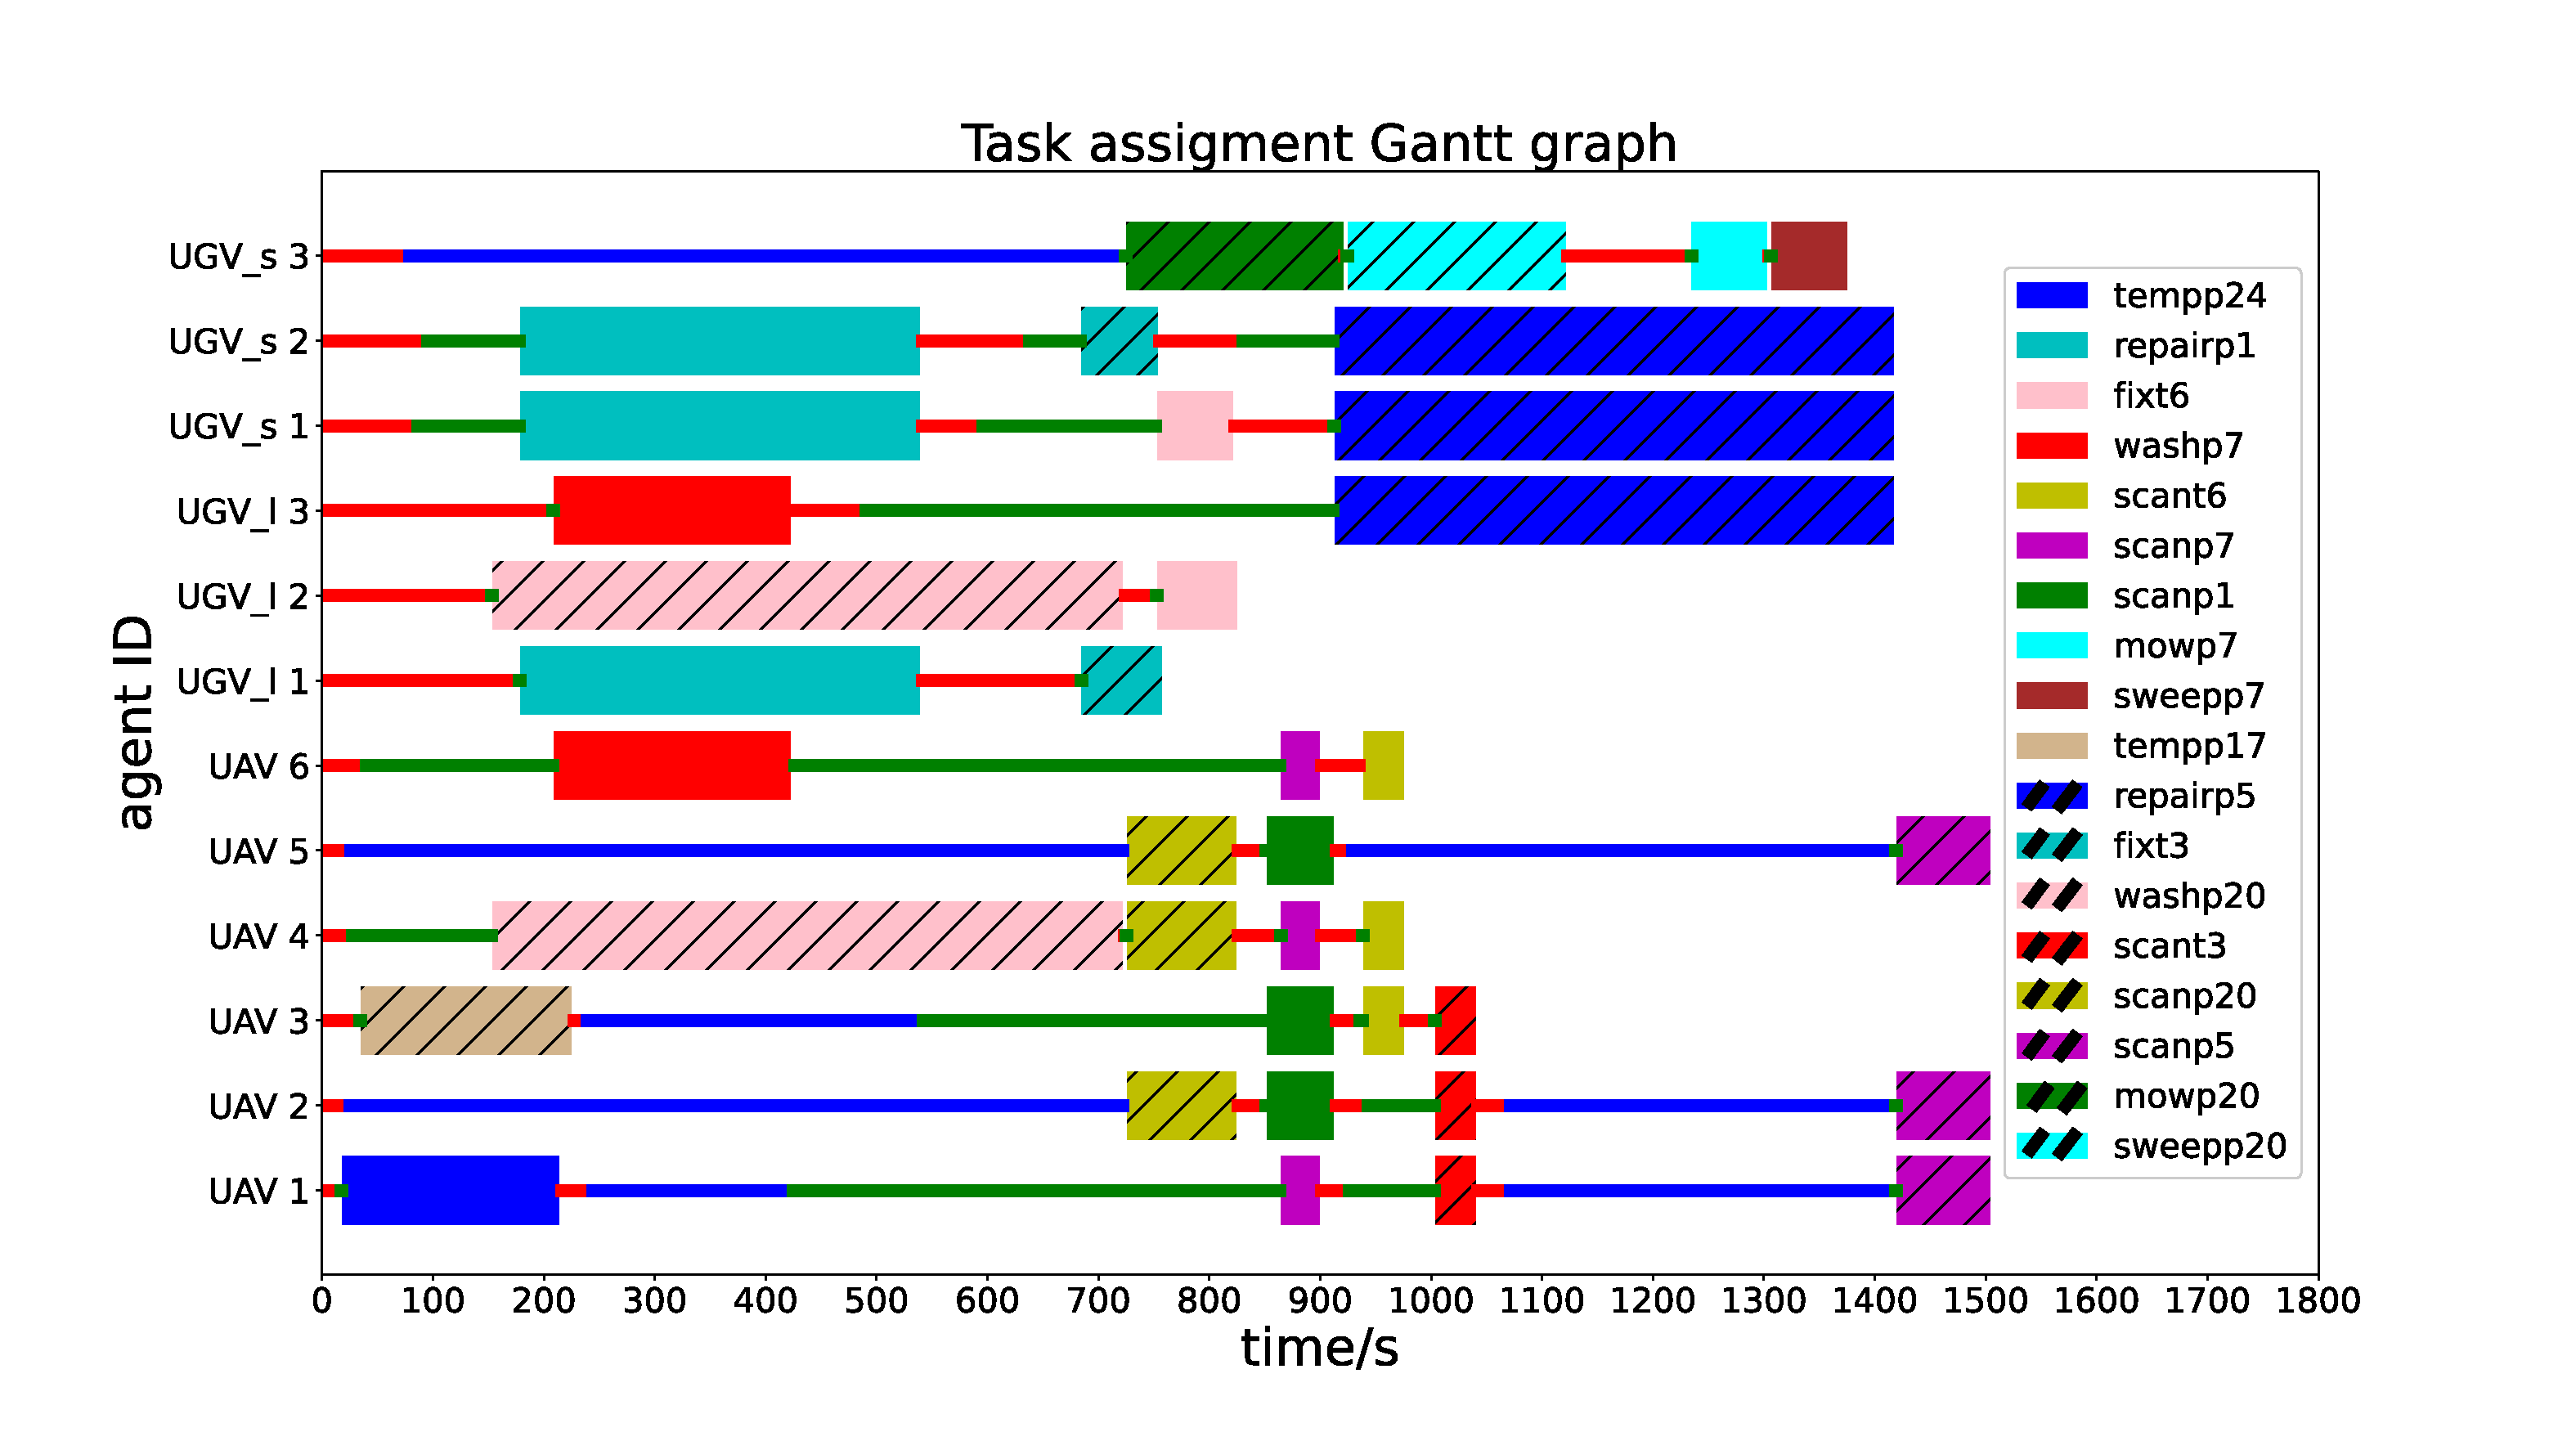
\includegraphics[scale=0.180]{figures/simulation/onlineadaptive/gantt_1_adapt.pdf}
	\caption{
Gantt graph of the plan execution under fluctuated subtask duration for task Three.
Additional lines are added to highlight the online synchronization process.
Red segments indicate that the agents are during transition among regions,
green segments for ``waiting for collaborators'',
and blue segments for ``waiting for preceding subtask in partial order''.}
	\label{fig:gantt-online-task3}
\end{figure}
%==============================

Notably, the associated MILP for the same problem consists of $38880$ Boolean variables,
which can not be solved within a reasonable time or memory.
In contrast, the proposed algorithm returns the first valid solution in $3.4s$,
and within~$5\%$ margin of the optimal value in $6.74s$.


%==============================
\subsubsection{Online Adaptation}\label{subsubsec:exp-adapt}
As an important part of the contribution, we now simulate
the following two practical scenarios to validate the proposed online adaptation algorithm.:
(i) fluctuations in the execution time of subtasks;
(ii) several agents break down during the online execution,

First of all, we artificially change the executing time of certain subtasks.
For instance, the executing time of the maintenance tasks for smaller panels
is reduced in comparison to the large panels, e.g., the execution time
of $\texttt{wash}_{\texttt{p}_7}$ are reduced to $212s$ from $565s$, as the size
of $\texttt{p}_1,\texttt{p}_3,\texttt{p}_6,\texttt{p}_7$ is $37.5\%$
of~$\texttt{p}_{10}$.
Consider the most complex task Three.
The proposed online synchronization method in Sec.~\ref{subsubsec:uncertain}
is applied during execution to dynamically accommodate these fluctuations.
Compared with the nominal case,
the execution result in Fig.~\ref{fig:gantt-online-task3} shows that the relative
ordering constraints are kept and the collaborative tasks are executed successfully.
Instead of following strictly the schedule in~$J^\star$, the agents rely on the
synchronization protocol.
For instance, since the task~$\texttt{wash}_{\texttt{p}_7}$ is finished earlier,
the subsequent task~$\texttt{mow}_{\texttt{p}_7}$ can be started immediately,
given the relation~$\texttt{wash}_{\texttt{p}_7} \leq \texttt{mow}_{\texttt{p}_7}$
and~$\texttt{wash}_{\texttt{p}_7} \neq \texttt{mow}_{\texttt{p}_7}$.
To give another example, vehicles~$V_{l_1}, V_{s_1},V_{s_2}$ are required to execute
task~$\texttt{repair}_{\texttt{p}_1}$.
Its exact schedule in~$J^\star$ is~$[173s,\, 746s]$, while actually it is started
at~$170s$ and finished at~$533s$, which is much earlier than scheduled.
Afterwards, all vehicles start immediately executing the subsequent subtasks
without waiting until~$746s$.
Similarly, vehicle~$V_{s_3}$ arrives at~$\texttt{p}_{20}$ at around~$72s$, but waits until
the subtask~$\texttt{wash}_{\texttt{p}_{20}}$ is finished at~$718s$,
in order to start executing the subtask~$\texttt{mow}_{\texttt{P}_{20}}$.
%==============================
\begin{figure}[t!]
	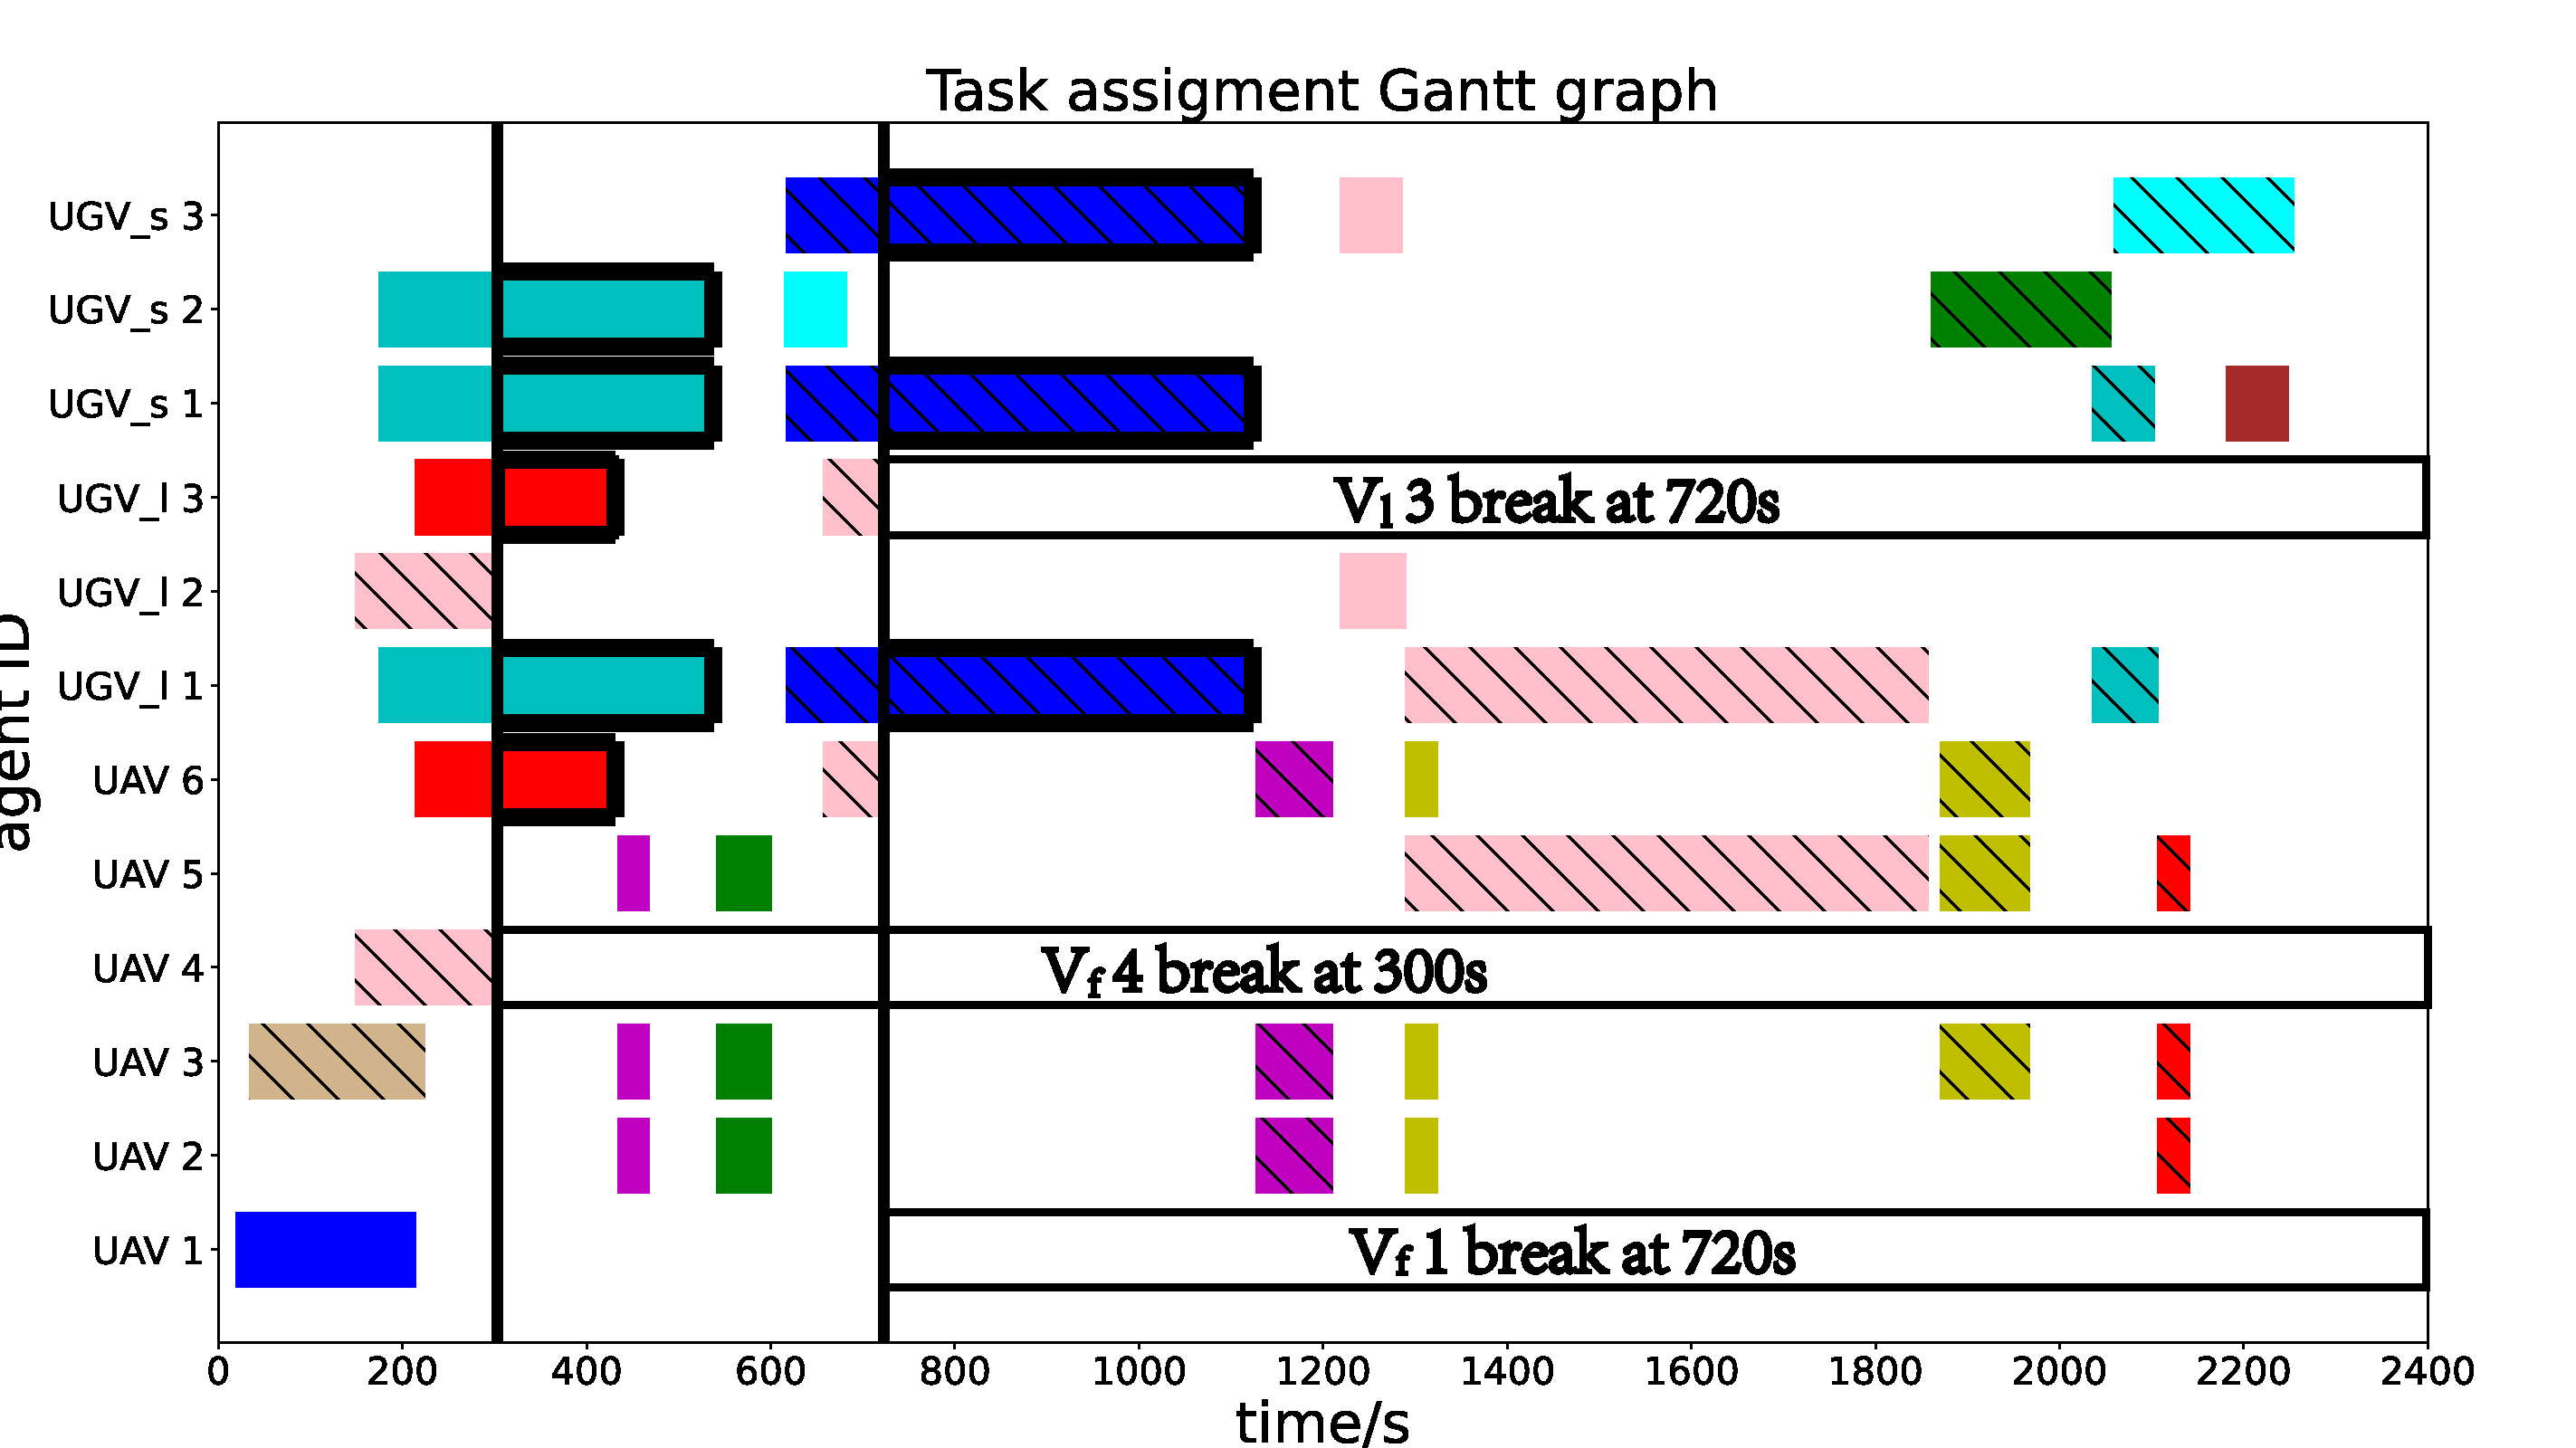
\includegraphics[scale=0.18]{figures/simulation/onlineadaptive/gantt_final_rebuild.pdf}
	\centering
	\caption{
Gantt graph of the plan execution under agent failures during the execution of task Three.
Three failures are highlighted in black.
Interrupted subtasks are repeated in the new-assignment.
The same legend for subtasks is shared with Fig.~\ref{fig:gantt-online-task3}.}
        \label{fig:online-failure-task3}
\end{figure}
%==============================


Secondly, more severe scenarios are simulated where agents break down
during task execution and thus are removed from the team.
More specifically, vehicle~$V_{f_4}$ breaks down at~$300s$, $V_{f_1},\, V_{l_3}$ break
down at~$720s$ during the execution of task Three.
Consequently, as shown in Fig.~\ref{fig:online-failure-task3},
the execution of subtask~$\texttt{wash}_{\texttt{p}_{20}}$ is interrupted at~$300s$.
As described in Sec.~\ref{subsubsec:failure},
the set of unfinished tasks is re-assigned to the remaining agents by re-identifying
the current node in the BnB search tree and continue the planning process.
It can be seen that no subtasks are assigned to~$V_{f_4}$ anymore in the updated assignment.
Moreover, the subtask~$\texttt{wash}_{\texttt{p}_{20}}$ is executed again
by vehicles~$V_{l_3}$ and $V_{f_6}$ at~$720s$.
Afterwards, since~$V_{f_1},\, V_{l_3}$ break down at~$720s$,
the execution of subtask~$\texttt{wash}_{\texttt{p}_{20}}$ is interrupted \emph{again} at~$720s$.
In the same way, the unfinished subtasks are re-assigned to the remaining agents.
Consequently, the subtask~$\texttt{wash}_{\texttt{p}_{20}}$ is executed again
by vehicles~$V_{l_1}$ and~$V_{f_5}$ at~$720s$ at~$1300s$.
It is worth noting that the partial ordering constraints are respected at all
time during the adaptation.
For instance, $V_{f_6}$ cannot execute the subtask~$\texttt{scan}_{\texttt{p}_5}$
before~$\texttt{repair}_{\texttt{p}_5}$ is finished,
as~$\texttt{scan}_{\texttt{p}_5}\neq_\varphi \texttt{repair}_{\texttt{p}_5}$ holds.
All subtasks are fulfilled at~$2141s$, despite of the above contingencies.



%==============================
\subsubsection{Scalability Analysis}\label{subsubsec:scalable}
To further validate the scalability of the proposed methods,
the following tests are performed:
(i) the same task with increased team sizes,
e.g., $8$, $16$, $24$, $32$ and $40$;
(ii) increased complexity of considered tasks, e.g.,
by adding more maintenance tasks at different regions.

As summarized in Table~\ref{table:more-agents},
as the system size is increased from~$8$ to $40$,
the computation time to obtain the \emph{first}
solution for task Three remains almost unchanged,
while the time taken to compute the optimal value increases slightly.
This result verifies that the proposed anytime algorithm is beneficial
especially for large-scale systems, as it can returns a high quality solution fast,
and close-to-optimal solutions can be returned as time permits.
Secondly, the subtasks~$\texttt{fix-scan}_{\texttt{t}_j}$ and $\texttt{repair-scan}_{\texttt{p}_i}$
within task Two is extended by adding more transformers and panels to maintain.
As summarized in Table~\ref{table:more-agents} right, the computation time of
both posets and tasks assignment are increased significantly, as the task becomes more
complex.
However, the time for the $10\%$ margin of the optimal solution does not monotonically
increase.
It is worth noting that as the number of tasks increases, the size of NBA explodes
such that the NBA pruning steps become infeasible.
Instead, the resulting poset of each subtask is composed algorithmically into the
complete set of posets.
Since the algorithm to compute the upper and lower bounds during the BnB search
has a complexity linear to the task complexity, the assignment algorithm
can still return the optimal value in proper time given the computed posets.
For example, for the extreme case of~$45$ subtasks when~$N_{\texttt{t}}=N_{\texttt{p}}=5$,
the first solution is found within~$0.58s$ while the close-to-optimal solution is
returned in~$3.26s$.


%==============================
\begin{table}[t]
  \centering
  \begin{threeparttable}
	\caption{Scalability analyses of the proposed method}
	\label{table:more-agents}
  \begin{tabular}{|c|c||c|c|}\hline
    \tnote{1} \begin{tabular}{@{}c@{}} System \\ $(V_f,V_s,V_l)$\end{tabular}
    &  \tnote{3} $t_{\texttt{sol}}\,[s]$
    & \tnote{2} \begin{tabular}{@{}c@{}} Task \\ $(N_{\texttt{t}},N_{\texttt{p}})$ \end{tabular}
    & \tnote{3} $t_{\texttt{sol}}\,[s]$  \\[0.5ex] \hline
		$(4,2,2)$  & $(0.50,1.57,2.84)$ &$(1,1)$ & $(0.03,0.17,0.21)$ \\[0.5ex]
		$(8,4,4)$ & $(0.47,1.73,3.91)$ &$(2,2)$ & $(0.09,0.53,1.38)$  \\[0.5ex]
		$(12,6,6)$ & $(0.44,2.03,5.53)$  & $(3,3)$ & $(0.20,1.21,4.65)$ \\[0.5ex]
		$(16,8,8)$  & $(0.50,1.18,4.08)$  & $(4,4)$ & $(0.35,1.09,13.29)$ \\[0.5ex]
		$(20,10,10)$  & $(0.53,1.39,3.67)$ & $(5,5)$ & $(0.58,3.26,36.15)$ \\ [0.5ex]
    \hline
  \end{tabular}
  \begin{tablenotes}
    \item[1] The number of different types of agents as system size increases.
    \item[2] The number of transformers and panels
      that should be serviced for maintenance in the task.
    \item[3] The associated solution time,
          measured by three time stamps when:
          the first solution is returned,
          the solution within~$10\%$ margin of the optimal solution is returned,
          and the optimal solution is returned.
  \end{tablenotes}
\end{threeparttable}
\end{table}
%==============================

%==============================
\subsubsection{Comparison}\label{subsubsec:compare}
The proposed method is compared against several
state-of-the-art methods in the literature.
More specifically, four methods below are compared:

\textbf{Prod}: the standard solution~\cite{baier2008principles}
that first computes
the Cartesian products of all agent models,
then computes the product B\"uchi automaton,
and searches for the accepting run within.
As the brute-force method,
it is well-known to suffer from complexity explosion.

\textbf{Milp}: the optimization-based solution that
formulates the assignment problem of posets as a MILP
the compute optimal assignment similar
to~\cite{luo2021temporal, jones2019scratchs},
i.e., instead of the search method.
The partial relations are formulated as constraints
in the program.
An open source solver GLPK~\cite{makhorin2008glpk} is used.

\textbf{Samp}: the sampling based method proposed
in~\cite{kantaros2020stylus}.
Compared with the product-based methods, it does not pre-compute
the complete system model. Instead it relies on a sampling strategy
to explore only relevant search space.
However, since it does not support collaborative actions natively,
we modify the definition of transitions there slightly.

\textbf{Decomp}: the task assignment strategy proposed
in~\cite{schillinger2018simultaneous}.
As discussed earlier in Sec.~\ref{sec:introduction},
the proposed task decomposition strategy only allows completely
independent subtasks.
Furthermore, since it does not support collaborative actions,
collaborative subtasks are decomposed manually.
%==============================
\begin{table}[t]
  \centering
  \begin{threeparttable}
	\caption{Comparison to other methods.}
	\label{table:compare}
	\begin{tabular}{|c|c|c|c|c|c|}\hline
	  \tnote{1} Method & \tnote{2} $t_{\texttt{first}}\, [s]$
          & \tnote{2} $t_{\texttt{opt}}\, [s]$
	  & \tnote{2} $t_{\texttt{final}}\,[s]$ & \tnote{2} $T_{\texttt{obj}}\,[s]$
          & \tnote{2} $N_{\texttt{sync}}$ \\[0.5ex] \hline
		\multirow{2}{*}{\textbf{Prod}}& $\infty$ & $\infty$ & $\infty$ & -- & -- \\[0.5ex]
                 & $\infty$ & $\infty$ & $\infty$ & -- & -- \\[0.5ex]
                \hline
		\multirow{2}{*}{\textbf{Milp}} & 2069.27 & 2069.27 & 2069.27 & 1058.47 & -- \\[0.5ex]
                &$\infty$ &$\infty$ & $\infty$ & -- & --  \\[0.5ex]
                \hline
		\multirow{2}{*}{\textbf{Samp}} & 328.59 & 1838.96 & $\infty$ & 1968.03 & 24 \\[0.5ex]
                 & 3280.68 &  16294.30 & $\infty$ & 1968.03 & 24 \\[0.5ex]
                \hline
		\multirow{2}{*}{\textbf{Decomp}} & 580.16 & 580.16 & 4581.3 & 1266.99 & 0 \\[0.5ex]
		 & 1151.24 & 1151.24 & 5082.07 & 1267.00 & 0 \\[0.5ex]
                \hline
		\multirow{2}{*}{\textbf{Ours}} & 24.81 & 25.26 & $\infty$ & 1058.47 & 8 \\[0.5ex]
                 & 28.12 & 37.40 & $\infty$ & 1058.47 & 8 \\[0.5ex]
		\hline
	\end{tabular}
  \begin{tablenotes}
  \item[1] For each method, the first row measures the time for the
    system of~$12$ agents while the second row for~$24$ agents.
  \item[2] The time to derive the first solution,
    the time to derive the optimal solution,
    the termination time, the objective as the task completion time,
and the number of synchronizations required.
  \end{tablenotes}
   \end{threeparttable}
\end{table}
%==============================

Two identical comparisons are performed under different system sizes,
namely $12$ and $24$ agents, to compare not only efficiency but also scalability.
To begin with, the nominal system of~$12$ agents under task~$\varphi_2$ is considered.
The above four methods are used to solve the same planning problem.
As summarized in Table.~\ref{table:compare},
the results are compared in the following four aspects:
the time to derive the first solution,
the time to derive the optimal solution,
the termination time, the optimal solution,
and finally the number of online synchronizations required.
Since the methods \textbf{Prod}, \textbf{Milp} and \textbf{Decomp} are not
anytime, the time to obtain  the first solution equals to the time
when the optimal solution is obtained.
It can be seen that the \textbf{Prod} failed to generate any solution
within~$11h$ as the system-wide product automaton for both cases
has more than $10^{19}$ states.
The \textbf{Milp} method is only applicable for small problems,
which returns the optimal solution in~$0.5h$ but fails to
return any solution within~$16h$ for the large problem.
The \textbf{Samp} method has the anytime property but it takes ten times
the time to generate
the first feasible solution, compared with our method.
In addition, since the subtasks are executed in sequence by the solution,
the actual time of task completion is significantly longer.
The \textbf{Decomp} method can solve both problems but the overall time
for task completion is longer than our results,
which matches our analyses in Remark~\ref{remark:compare-poset}.
In comparison, our method returns the first solution for both cases in less
than~$30s$ and the optimal solution within another~$10s$.
It can be seen that the task completion time remains the same for both cases,
which is consistent with the \textbf{Milp} method.

Last but not least, the last column in Table~\ref{table:compare} compares the number
of synchronizations required during execution.
Although the same solution is obtained, the \textbf{Milp} method requires more
synchronization during execution than our method.
This is because our method requires only synchronization for relations within the
posets, rather than all consecutive subtasks.
The \textbf{Prod} and \textbf{Samp} methods require more synchronization due to
its fully sequential execution,
while the \textbf{Decomp} requires no synchronization as
the local subtasks of each agent are independent.
